\section{experimental evaluation}\label{sec:exp}
In this section, we conduct extensive experiments by comparing the proposed hash table designs with several state-of-the-art approaches for GPU-based hash tables. 
We will introduce the experimental setup and the discuss the results. 

\subsection{Experiment Setup}

\vspace{1mm}\noindent\textbf{Baselines.} We compare the proposed approach in this paper with several state-of-the-art hash table implementations on GPUs and CPUs. 
\begin{itemize}
	\item \cudpp is a popular CUDA primitive library which contains the hash table implementation published in~\cite{alcantara2009real}. 
	\cudpp employs three hashing function and each hash value stores only one KV pair with 64 bits size (32 bits for key and 32 bits for value). 
	Note that \cudpp only supports \formal{insert} and \formal{find} operations. 
	\item \megakv is a state-of-the-art approach for GPU-based key value store published in~\cite{zhang2015mega}. It employs a cuckoo hash with two hash functions.
	\megakv also allocates a basket for each hash value. However, it does not lock a basket when performing update. Instead, it uses intra-block synchronization to resolve race condition. 
	\item \linear is a GPU-based hash table which uses linear open addressing to resolve conflicts \cite{hong2010mapcg}. 
	\item \google is an efficient CPU-based hash table implementation\footnote{https://github.com/sparsehash/sparsehash-c11/}. We choose the \emph{dense\_hash\_map} implementation since it provides the best efficiency.
	\item \voter is the approach proposed in this paper.
\end{itemize}
We adopt the original implementations of \cudpp and \google from their corresponding inventors. 
For \megakv, we note that its intra-block synchronization could lead to inconsistency issue as well as a large number of insertion failures, especially when the filled ratio is high.  
Thus, we revise its code by replacing the intra-block synchronization with atomicExch to resolve the race condition. The adoption of atomicExch preserves the design principle of \megakv for \emph{not} locking the entire basket for updates. Moreover, it leads to less insertion failures and similar performance against its original implementation. 
For \linear, we implement the CUDA version of the algorithm proposed in \cite{hong2010mapcg}.
Note that we do not compare with the dynamic GPU hash approach proposed in \cite{ashkiani2018dynamic} for two major reasons. First, we cannot obtain the original implementation from its authors. Second, the approach devises a dedicated memory allocator other than cudaMalloc. A dedicated allocator will improve the performance but add complexity the system. Additionally, it needs to occupy a large memory in advance and is not transparent to other GPU applications.
In contrast, our proposed approach only use native allocator supported. 
We do not compare with \cite{breslow2016horton} since it only improves \megakv marginally using a more costly insertion process.

\begin{table}[t]
	\caption{The datasets used in the experiments.}
	\label{table:exp_data_sets}
	\centering
	\begin{tabular}{|c|c|c|c|}
		\hline
		Datasets & KV pairs & Unique keys & Size \\ \hline
		\dstwitter & & & \\ \hline
		\dsreddit & & & \\ \hline
		\dstpch & & & \\ \hline
		\dsali & & & \\ \hline
		\dsrandom & & & \\ \hline
	\end{tabular}
\end{table}

\vspace{1mm}\noindent\textbf{Datasets.} We evaluate all compared approaches using several real world and synthetic datasets described as follows:
\begin{itemize}
	\item \dstwitter: Twitter is an online social network where users perform actions include \emph{tweet}, \emph{retweet}, \emph{quote} and \emph{reply}.
	We crawl these actions for one week via Twitter stream API\footnote{https://dev.twitter.com/streaming/overview} on trending topics US president election, 2016 NBA finals and Euro 2016. The dataset contains 2,881,154 distinct users as keys and 9,724,908 actions.
	\item \dsreddit: Reddit is an online forum where users perform actions include \emph{post} and \emph{comment}. We collect all Reddit \emph{comment} actions in May 2015 from \emph{kaggle}\footnote{https://www.kaggle.com.reddit/reddit-comments-may-2015} and query the Reddit API for the \emph{post} actions the same period. The dataset contains 2,628,904 distinct users as keys and 48,104,875 actions. 
 	\item \dstpch: Lineitem is a synthetic table generated by the TPC-H benchmark\footnote{https://github.com/electrum/tpch-dbgen}. We generate \xxx rows of the lineitem table and select its partkey column and quantity column as the KV pairs. The dataset contains \xxx unique keys.  
	\item \dsali: \todo[inline]{Need to fill in the info for the dataaset.} The dataset contains \xxx unique products as keys and \xxx transactions. 
	\item \dsrandom: Random is a synthetic dataset generated from a normal distribution. 
	\todo[inline]{With what parameter?}
\end{itemize}

\begin{table}
	\centering
	\caption{Parameters in the experiments}
	\label{tbl:parameters}
	\begin{tabular}{|c|c|c|}
		\hline
		\textbf{Parameter} & \textbf{Settings} & \textbf{Default} \\ \hline
		$\alpha$ & 25\%, 30\%, 35\%, 40\%, 45\% & 40\% \\ \hline
		$\beta$  & 75\%, 80\%, 85\%, 90\%, 95\% & 90\% \\ \hline
		$r$ & 0.1, 0.2, 0.3, 0.4, 0.5 & 0.4 \\ \hline
	\end{tabular}
\end{table}

\vspace{1mm}\noindent\textbf{Static Hashing Comparison (Section~\ref{sec:exp:static}).}
Under the static setting, we evaluate \formal{insert} and \formal{find} performance among all compared approaches. 
In particular, we insert all KV pairs from the datasets followed by issuing 1 million random search queries. 

\vspace{1mm}\noindent\textbf{Dynamic Hashing Comparison (Section~\ref{sec:exp:dynamic}).}
Under the dynamic setting, we generate the workloads by batching the hash table operations. 
We partition the datasets into batches of $1$ million insertions. 
For each batch, we augment $1$ million \formal{find} operations and $1 \cdot r$ million \formal{delete} operations,
where $r$ is a parameter to balance insertions and deletions.
After we exhaust all the batches obtained from the datasets, we rerun these batches by swapping the \formal{insert} and \formal{delete} operations in any batch. 
We evaluate the performance of all compared approaches except \cudpp as it does not support deletions. 
Since all approaches other than \voter are static hash tables, we double/half the memory usage followed by rehashing all KV pairs as their resizing strategy, if the corresponding filled factor falls out of the specified range. 
Moreover, if an insertion failure is found for a compared approach, we trigger its resizing strategy.


\vspace{1mm}\noindent\textbf{Parameters.}
We vary the parameters when comparing \voter with the baselines.
$\alpha$ is the lower bound on the filled factor $\theta$ for all compared approaches,
whereas $\beta$ is the respective upper bound.
$r$ is the ratio of insertions over deletions in a processing batch. 
The settings of the aforementioned parameters could be found in Table~\ref{tbl:parameters}.

\vspace{1mm}\noindent\textbf{Experiment Environment.}
\todo[inline]{Fill in system specs.}

\subsection{Tunning Parameters}
\vspace{1mm}\noindent\textbf{Varying the number of hash tables.}

\begin{figure}[h]
\begin{minipage}{0.45\linewidth}\centering
	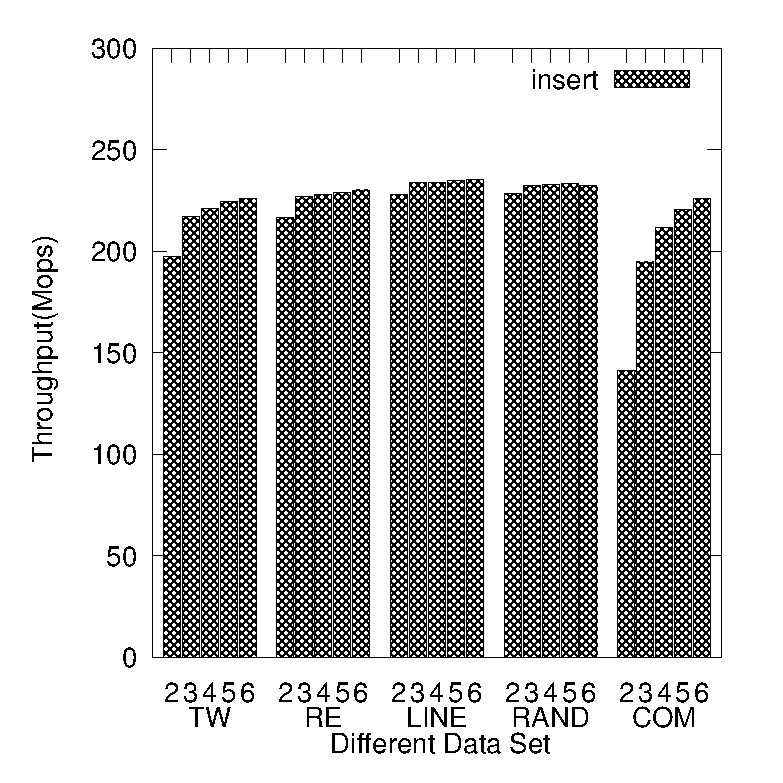
\includegraphics[width=\linewidth]{pic/tunning/tunning-insert.eps}
	\centerline{\formal{insert}}
	\end{minipage}
	\hfill
	\begin{minipage}{0.45\linewidth}\centering
	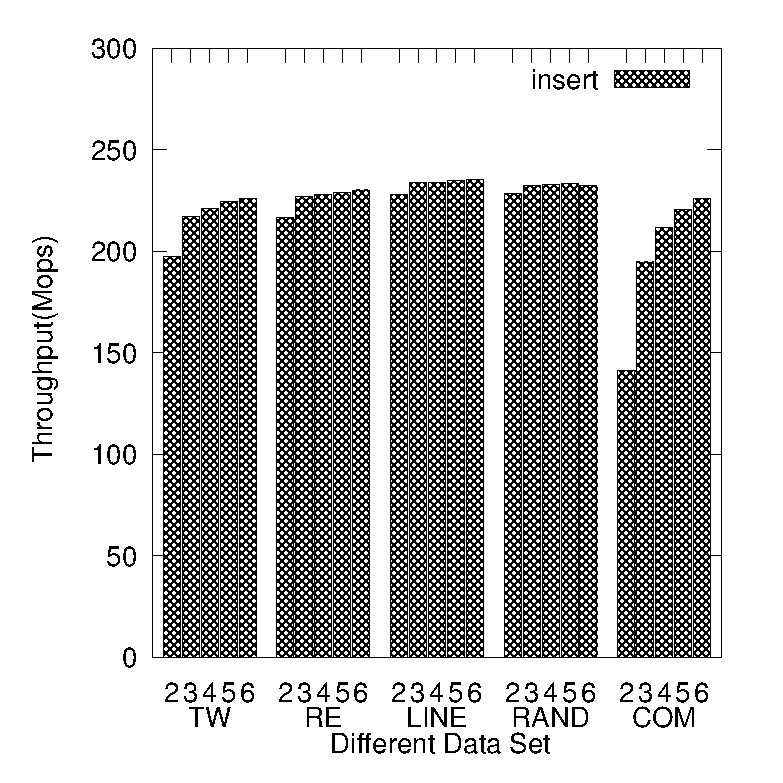
\includegraphics[width=\linewidth]{pic/tunning/tunning-insert.eps}
	\centerline{\formal{find}}
	\end{minipage}
	\caption{Throughput of \voter when varying number of hash tables.}
	\label{fig:vary-table}
\end{figure}

\subsection{Static Hashing Comparison}\label{sec:exp:static}
\vspace{1mm}\noindent\textbf{Varying the data variance $\sigma$.}

\begin{figure}[h]
	\begin{minipage}{0.45\linewidth}\centering
	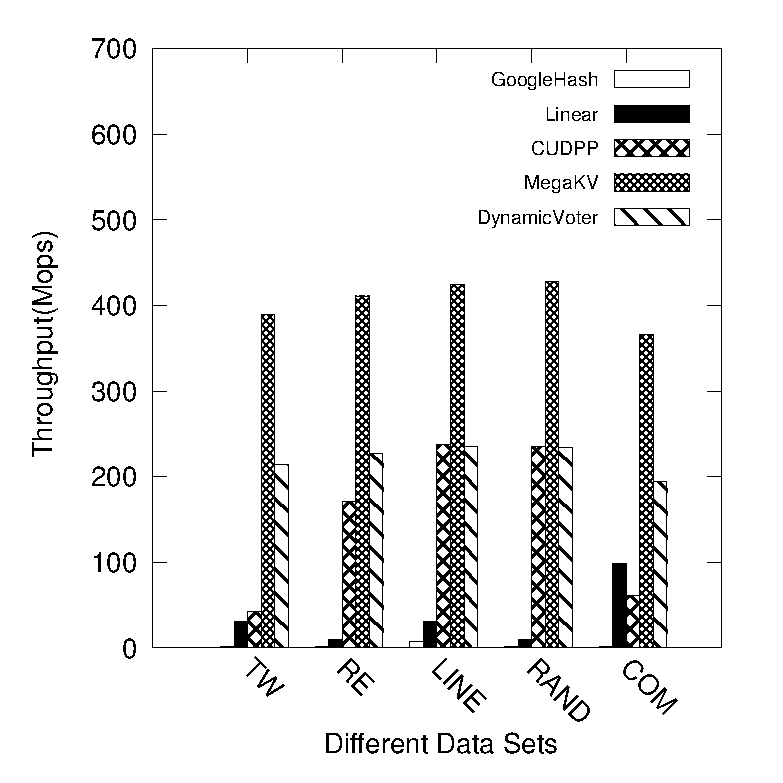
\includegraphics[width=\linewidth]{pic/static/static_insert.eps}
	\centerline{\formal{insert}}
	\end{minipage}
	\hfill
	\begin{minipage}{0.45\linewidth}\centering
	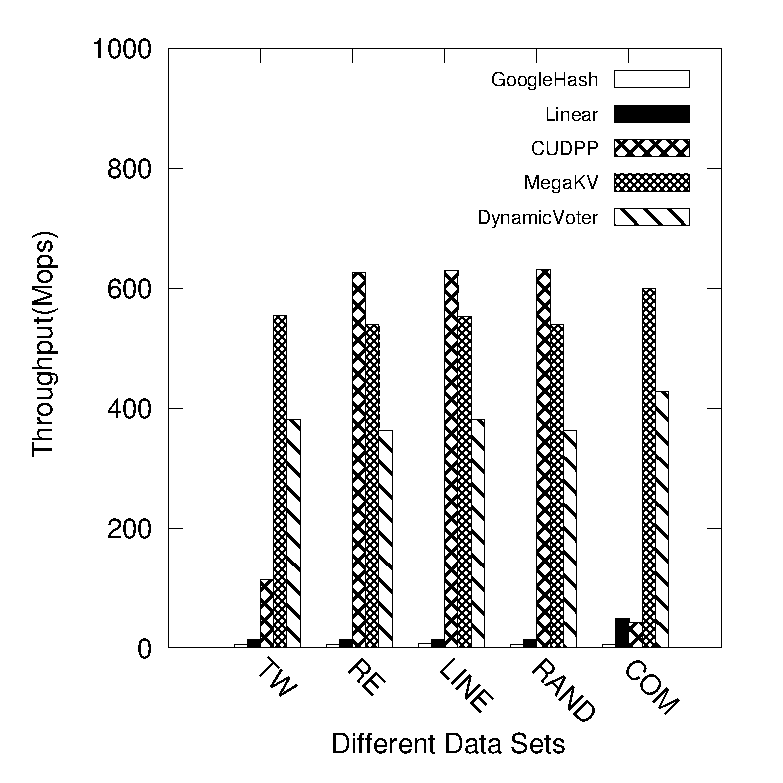
\includegraphics[width=\linewidth]{pic/static/static_search.eps}
	\centerline{\formal{find}}
	\end{minipage}
	\caption{Throughput of all compared approaches under the static setting.}
	\label{fig:static}
\end{figure}

\begin{figure*}[h]
	\begin{minipage}{0.3\linewidth}\centering
		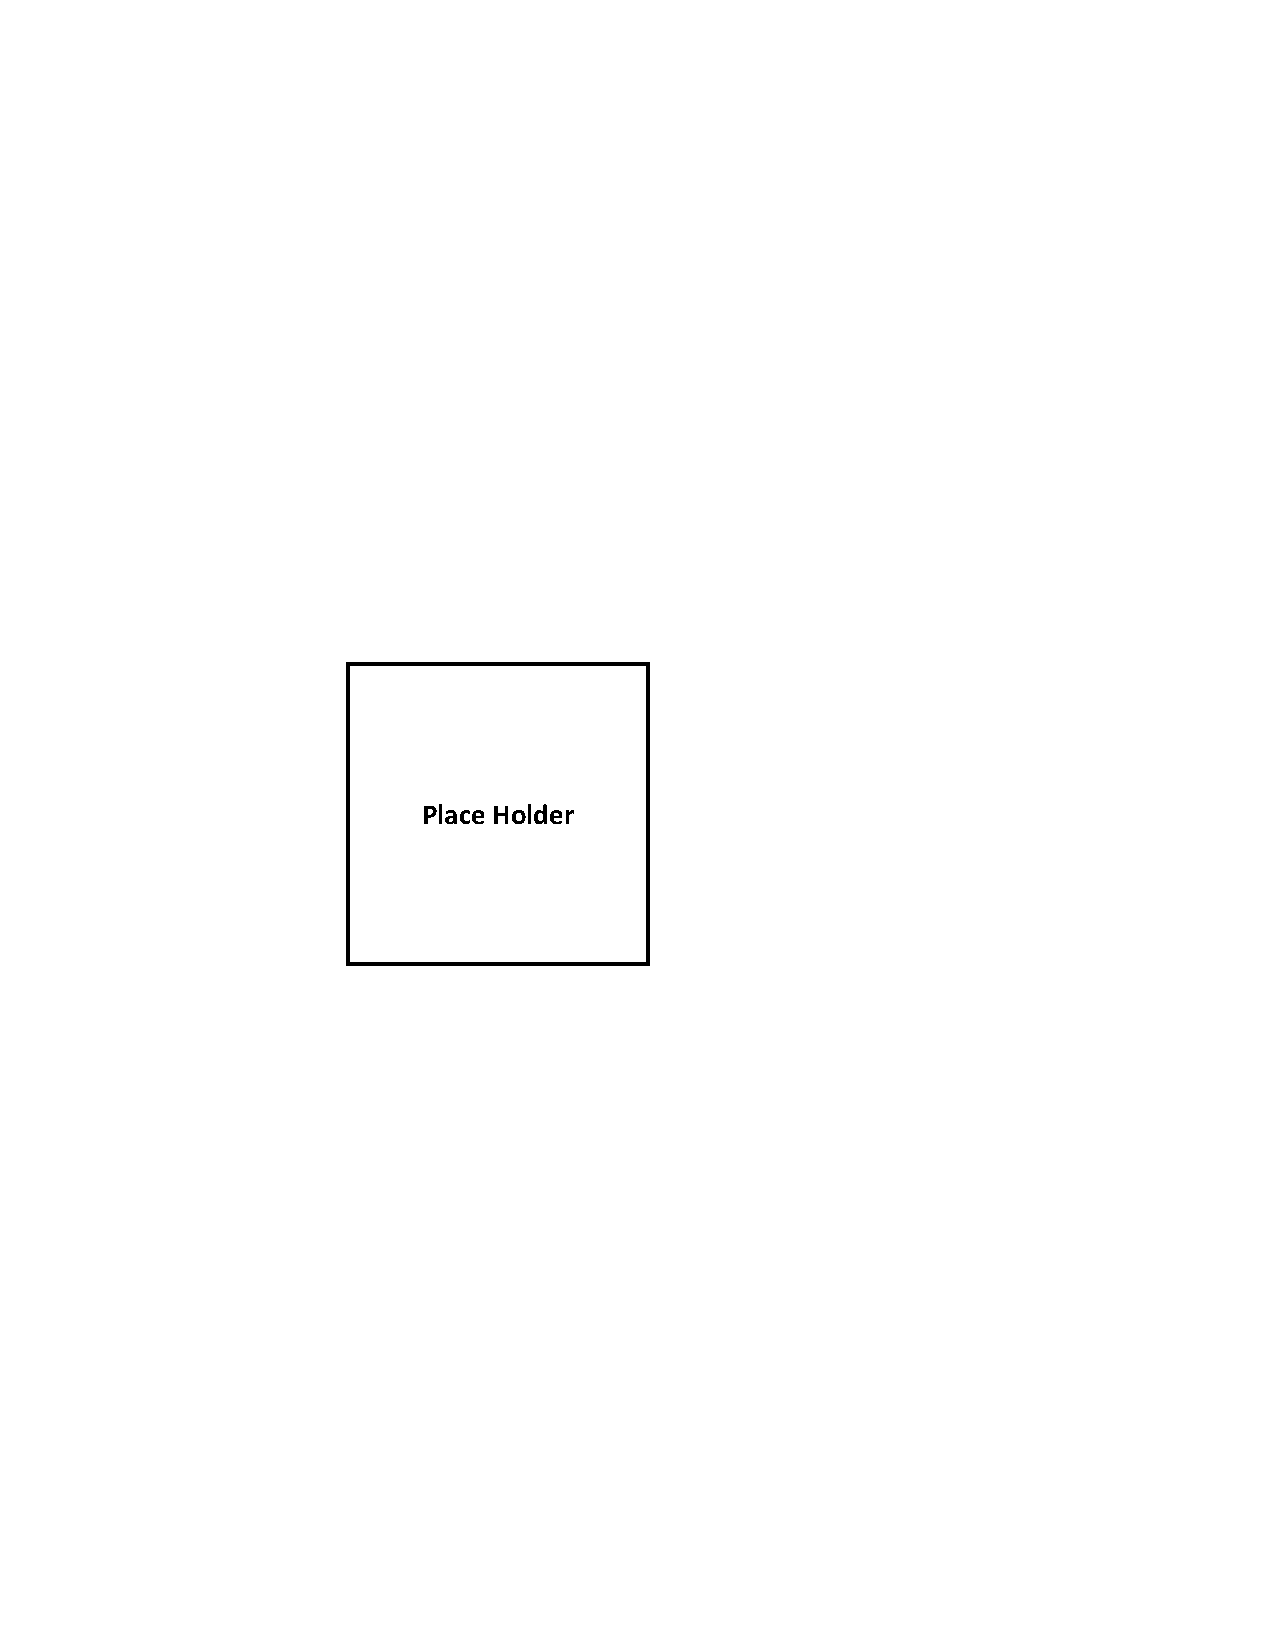
\includegraphics[width=\linewidth]{fig/PlaceHolder.pdf}
		\centerline{Warp Efficiency}
	\end{minipage}
	\hfill
	\begin{minipage}{0.3\linewidth}\centering
	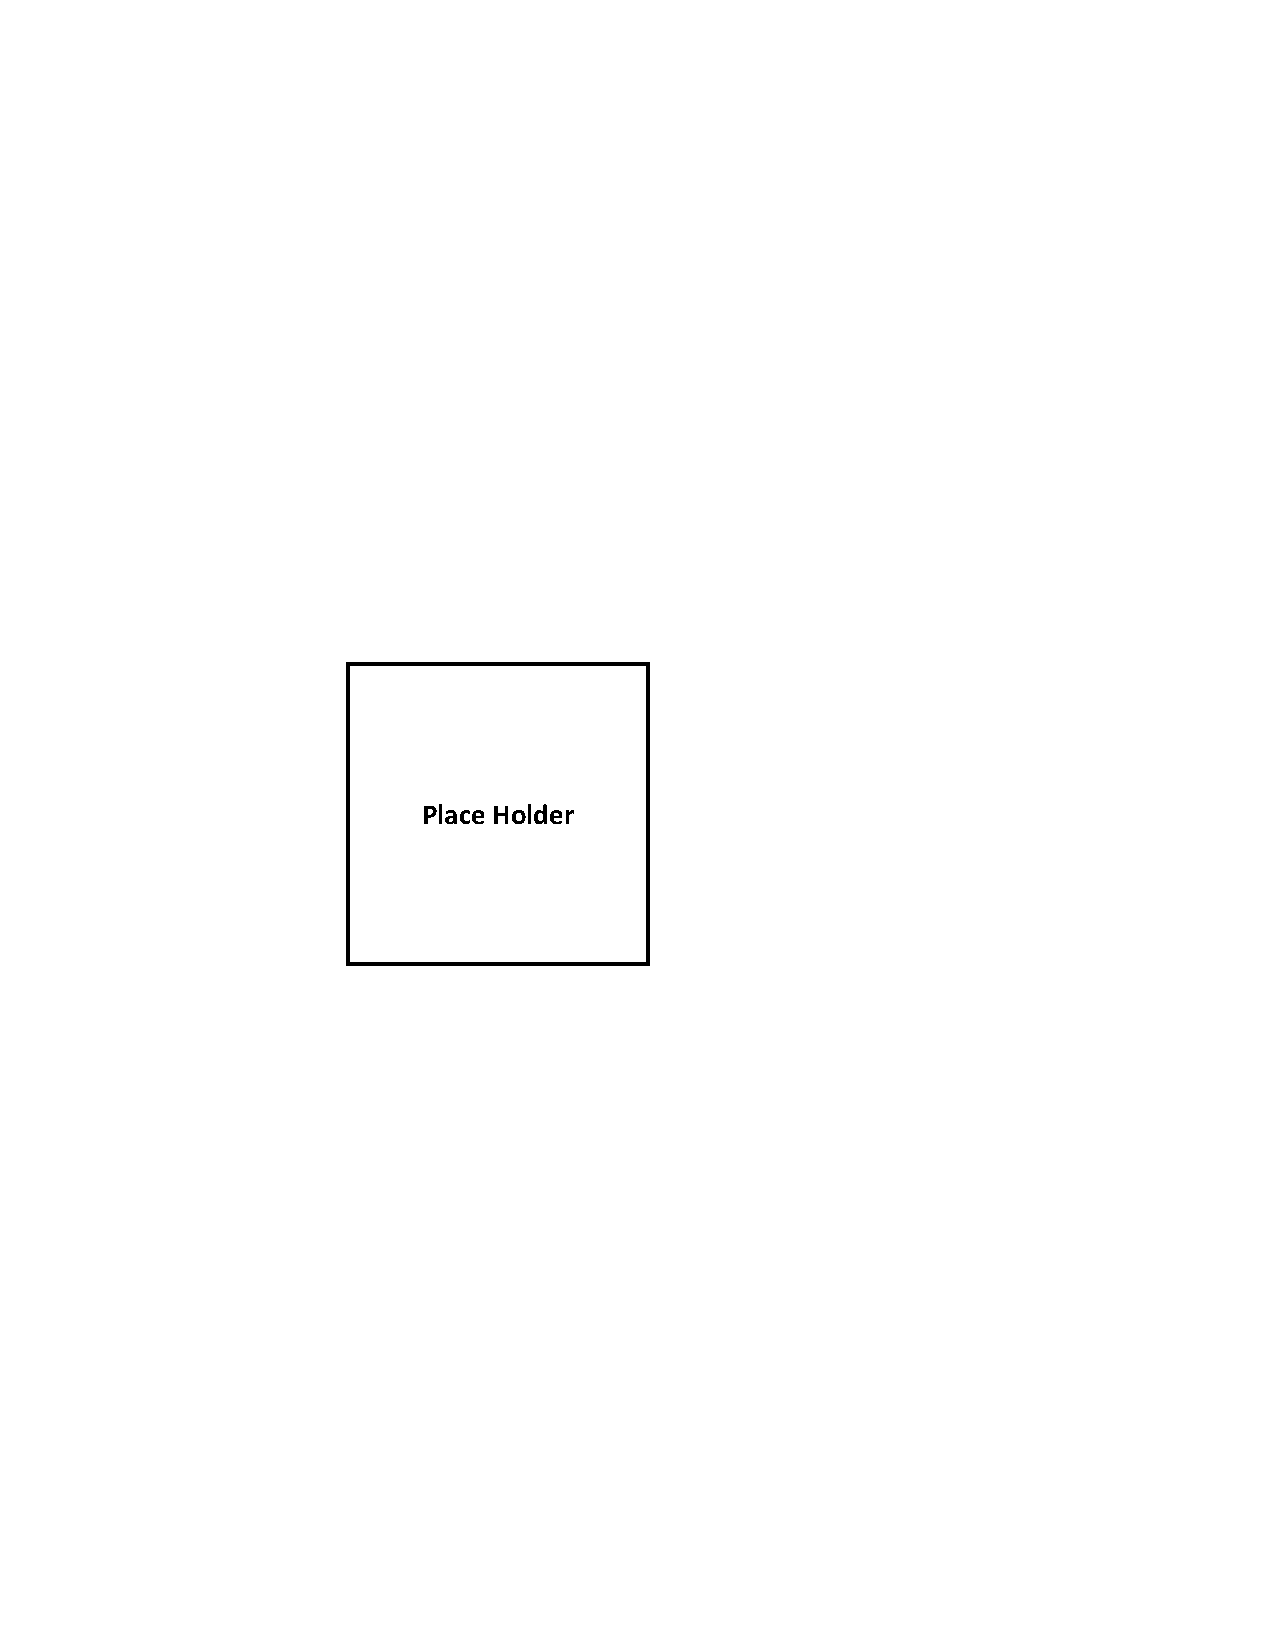
\includegraphics[width=\linewidth]{fig/PlaceHolder.pdf}
	\centerline{Memory Bandwidth Utilization}
	\end{minipage}
	\hfill
	\begin{minipage}{0.3\linewidth}\centering
	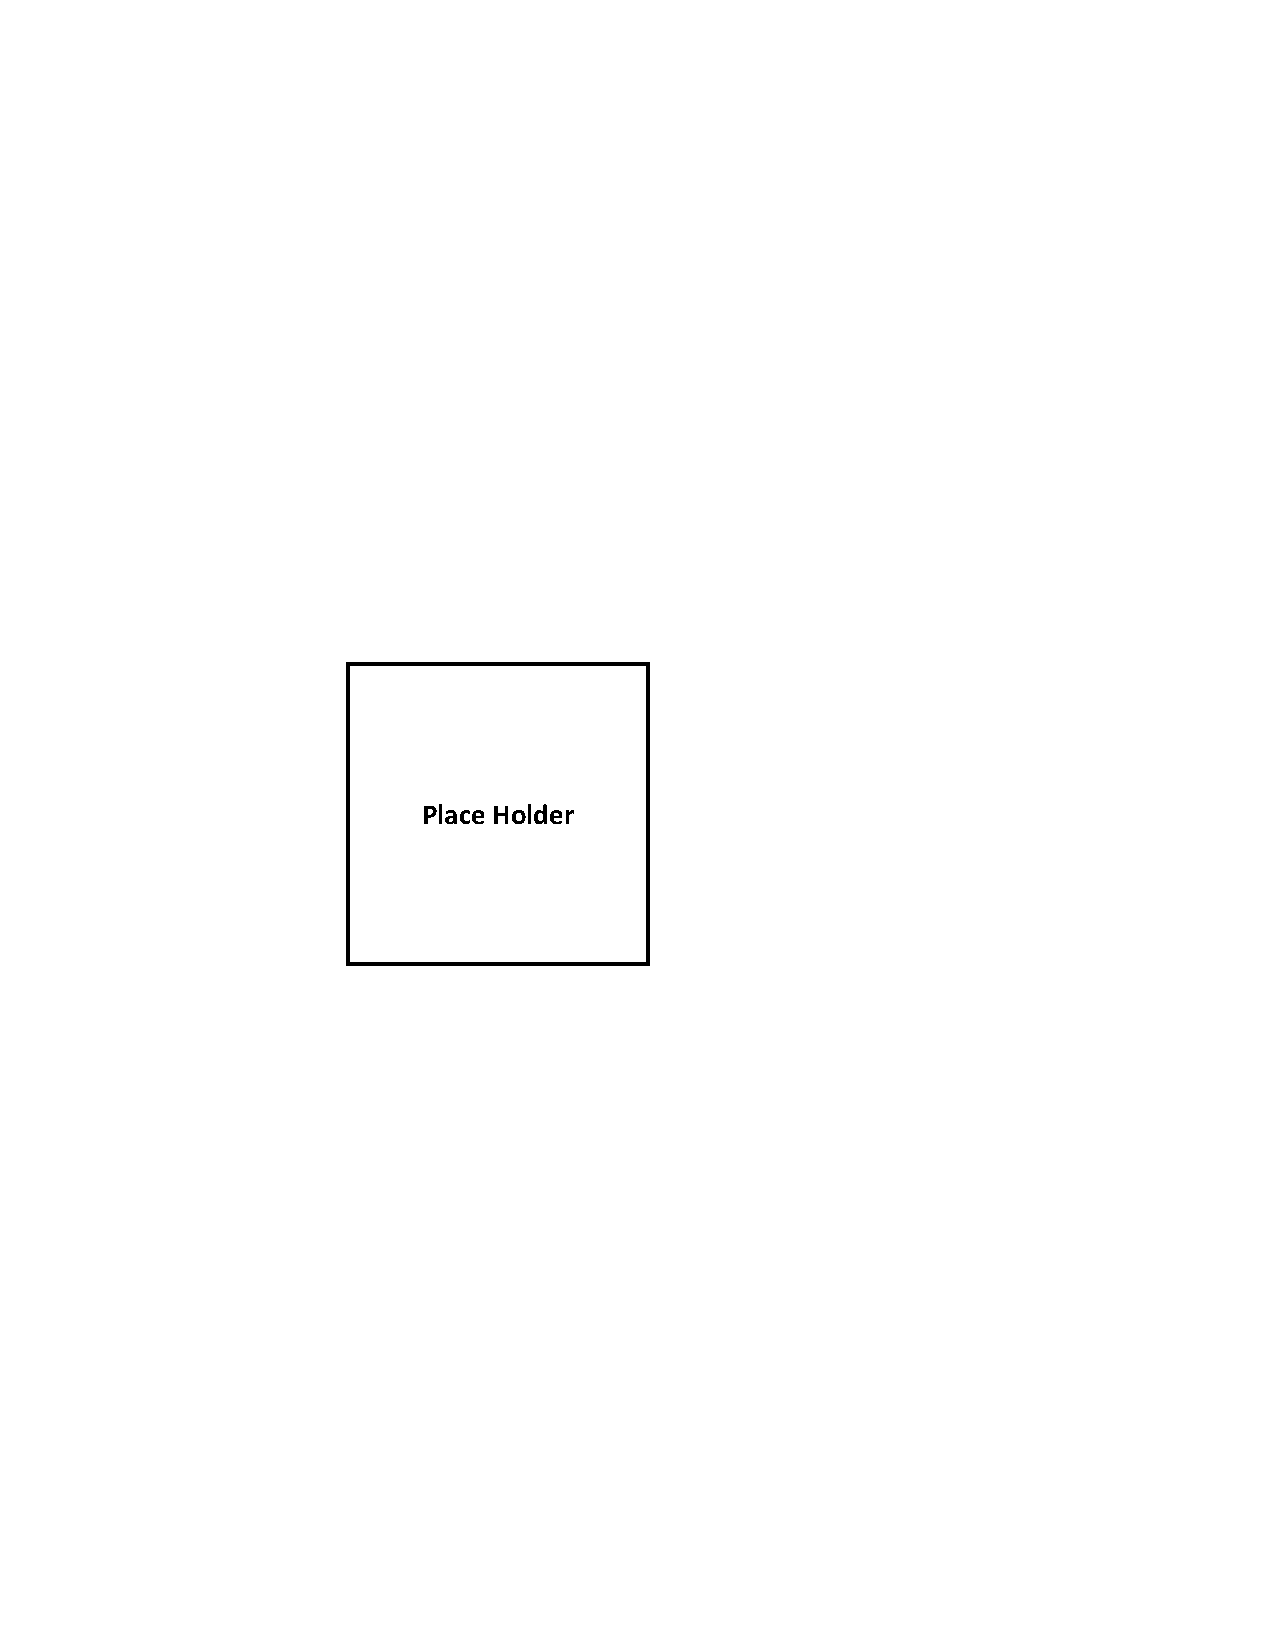
\includegraphics[width=\linewidth]{fig/PlaceHolder.pdf}
	\centerline{Cache Utilization}
	\end{minipage}
	\caption{Profiling the \formal{insert} performance for all compared approaches when varying the standard deviation $\sigma$.}
	\label{fig:static}
\end{figure*}

\subsection{Dynamic Hashing Comparison}\label{sec:exp:dynamic}

\vspace{1mm}\noindent\textbf{Varying the filled factor lower bound $\alpha$.}

\begin{figure*}[h]
	\begin{minipage}{0.18\linewidth}\centering
		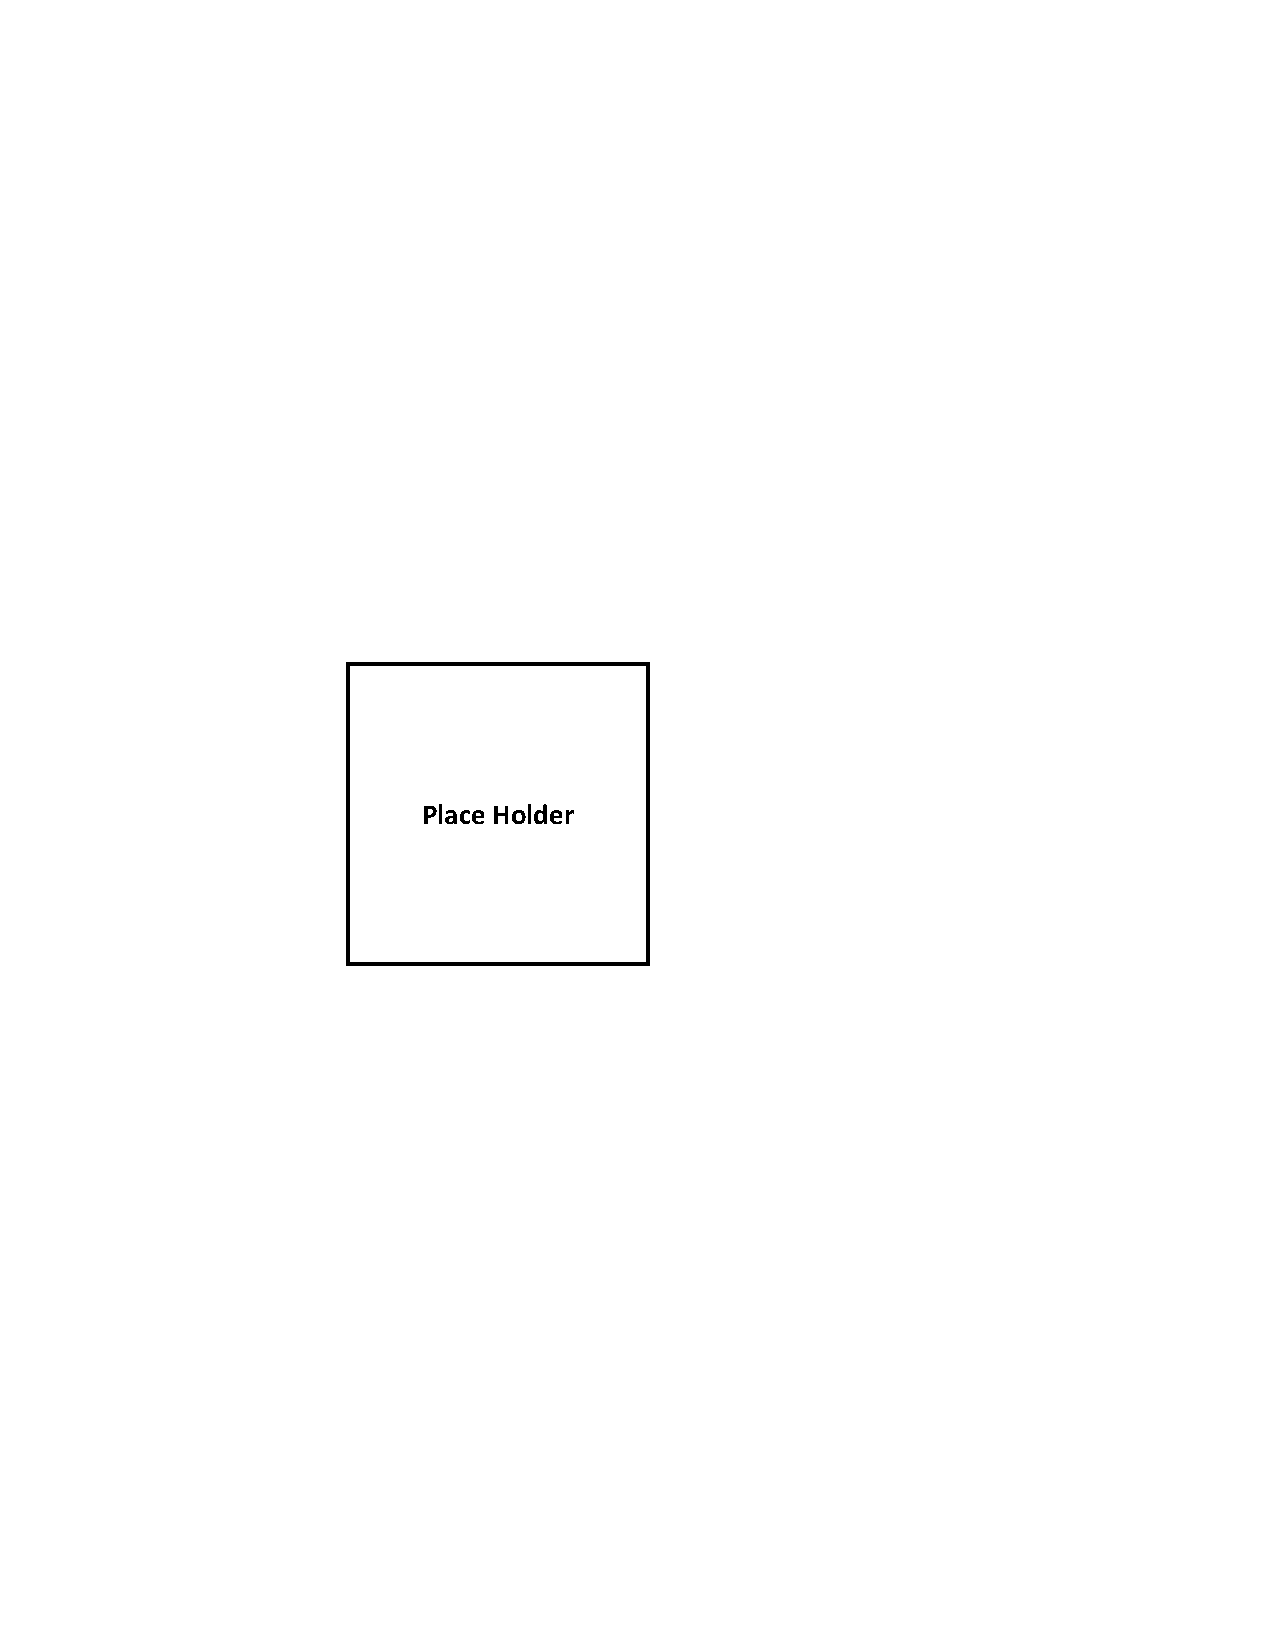
\includegraphics[width=\linewidth]{fig/PlaceHolder.pdf}
		\centerline{\dstwitter}
	\end{minipage}
	\hfill
	\begin{minipage}{0.18\linewidth}\centering
		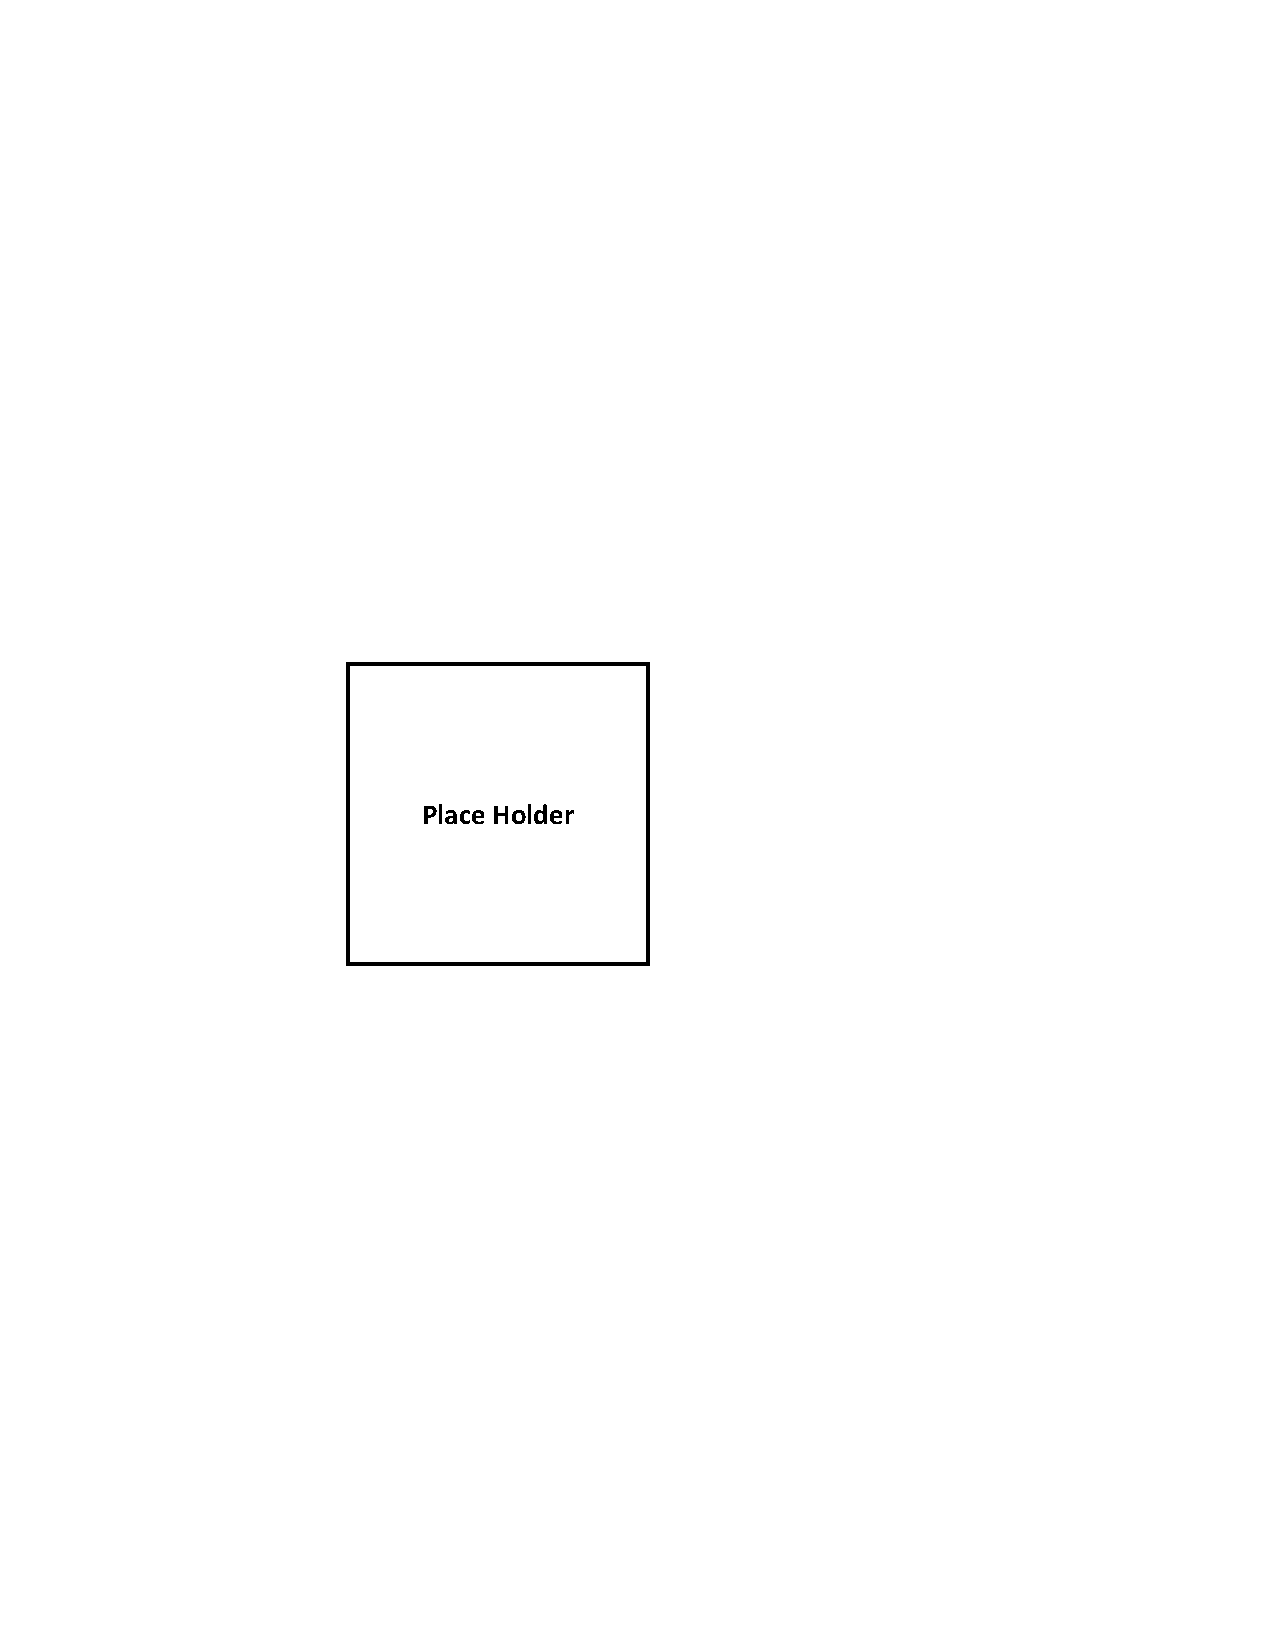
\includegraphics[width=\linewidth]{fig/PlaceHolder.pdf}
		\centerline{\dsreddit}
	\end{minipage}
	\hfill
	\begin{minipage}{0.18\linewidth}\centering
		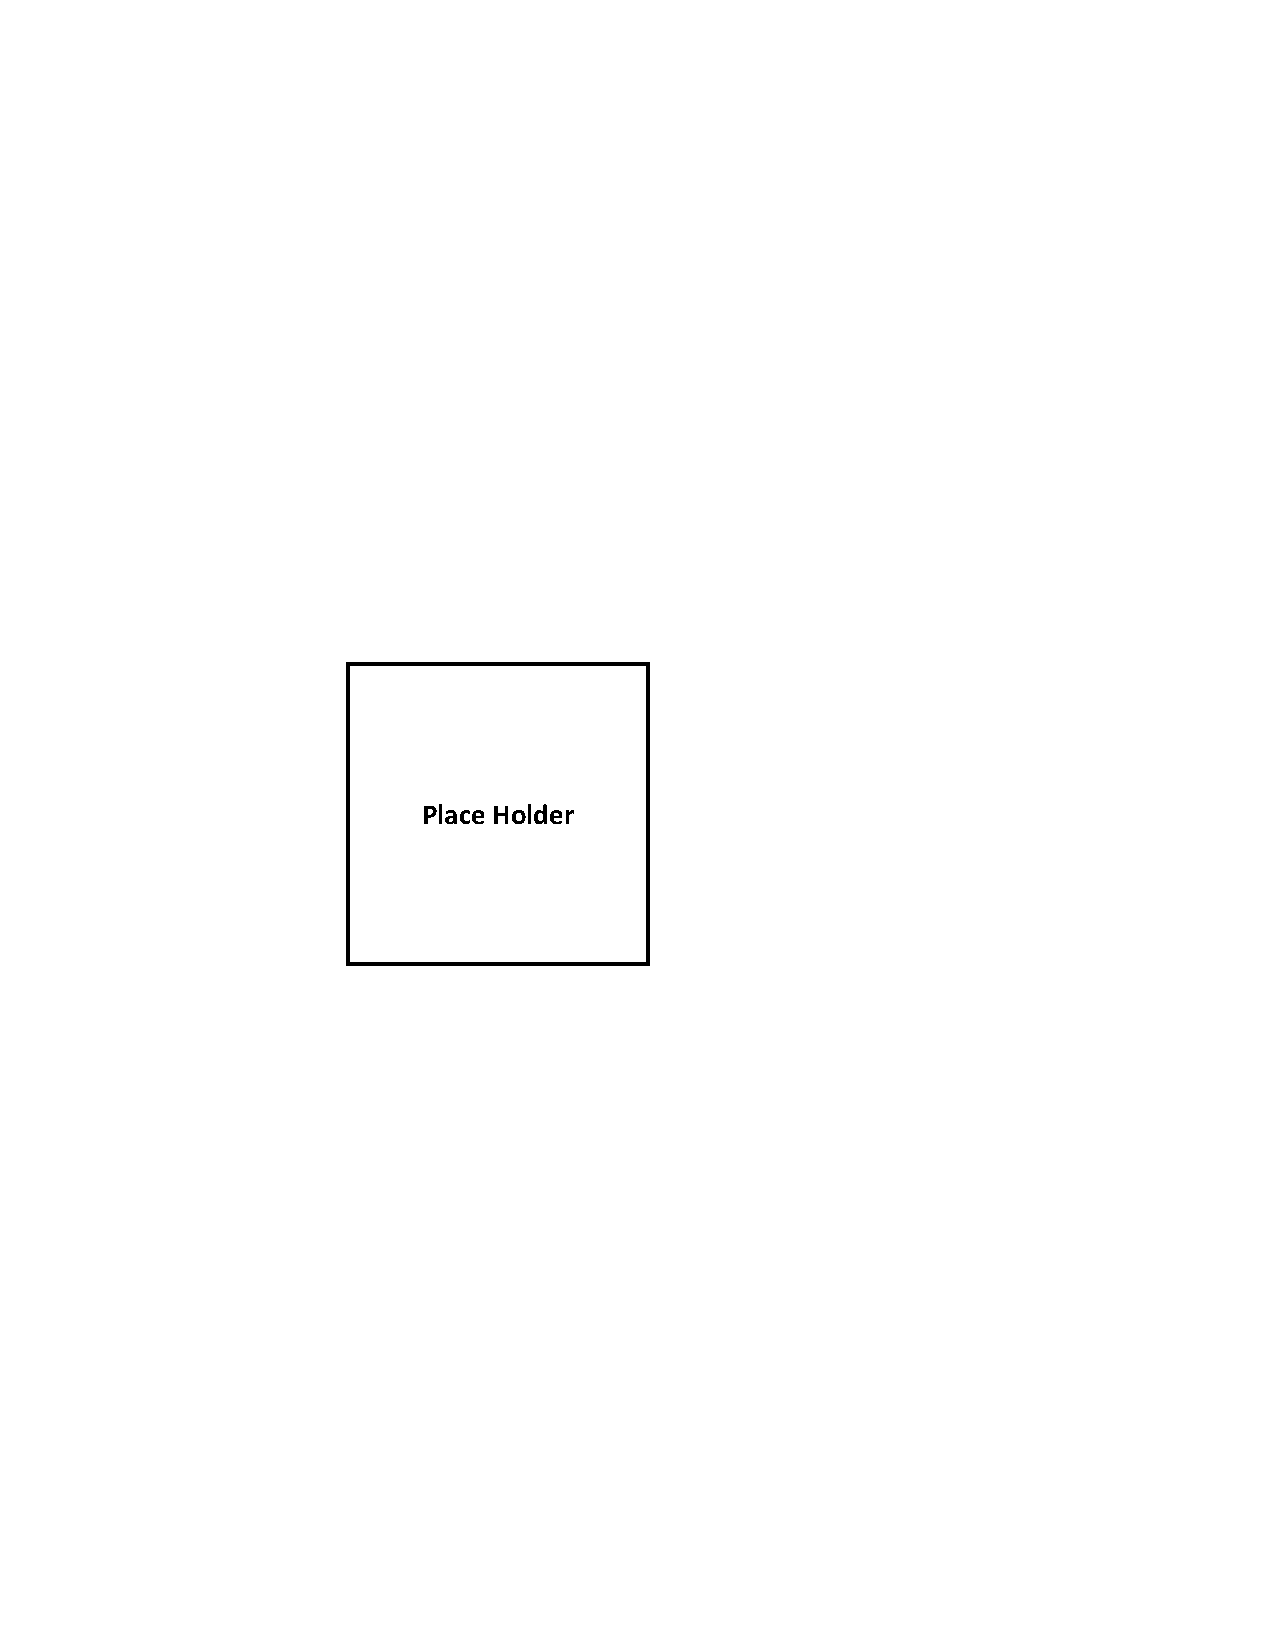
\includegraphics[width=\linewidth]{fig/PlaceHolder.pdf}
		\centerline{\dstpch}
	\end{minipage}
	\hfill
	\begin{minipage}{0.18\linewidth}\centering
		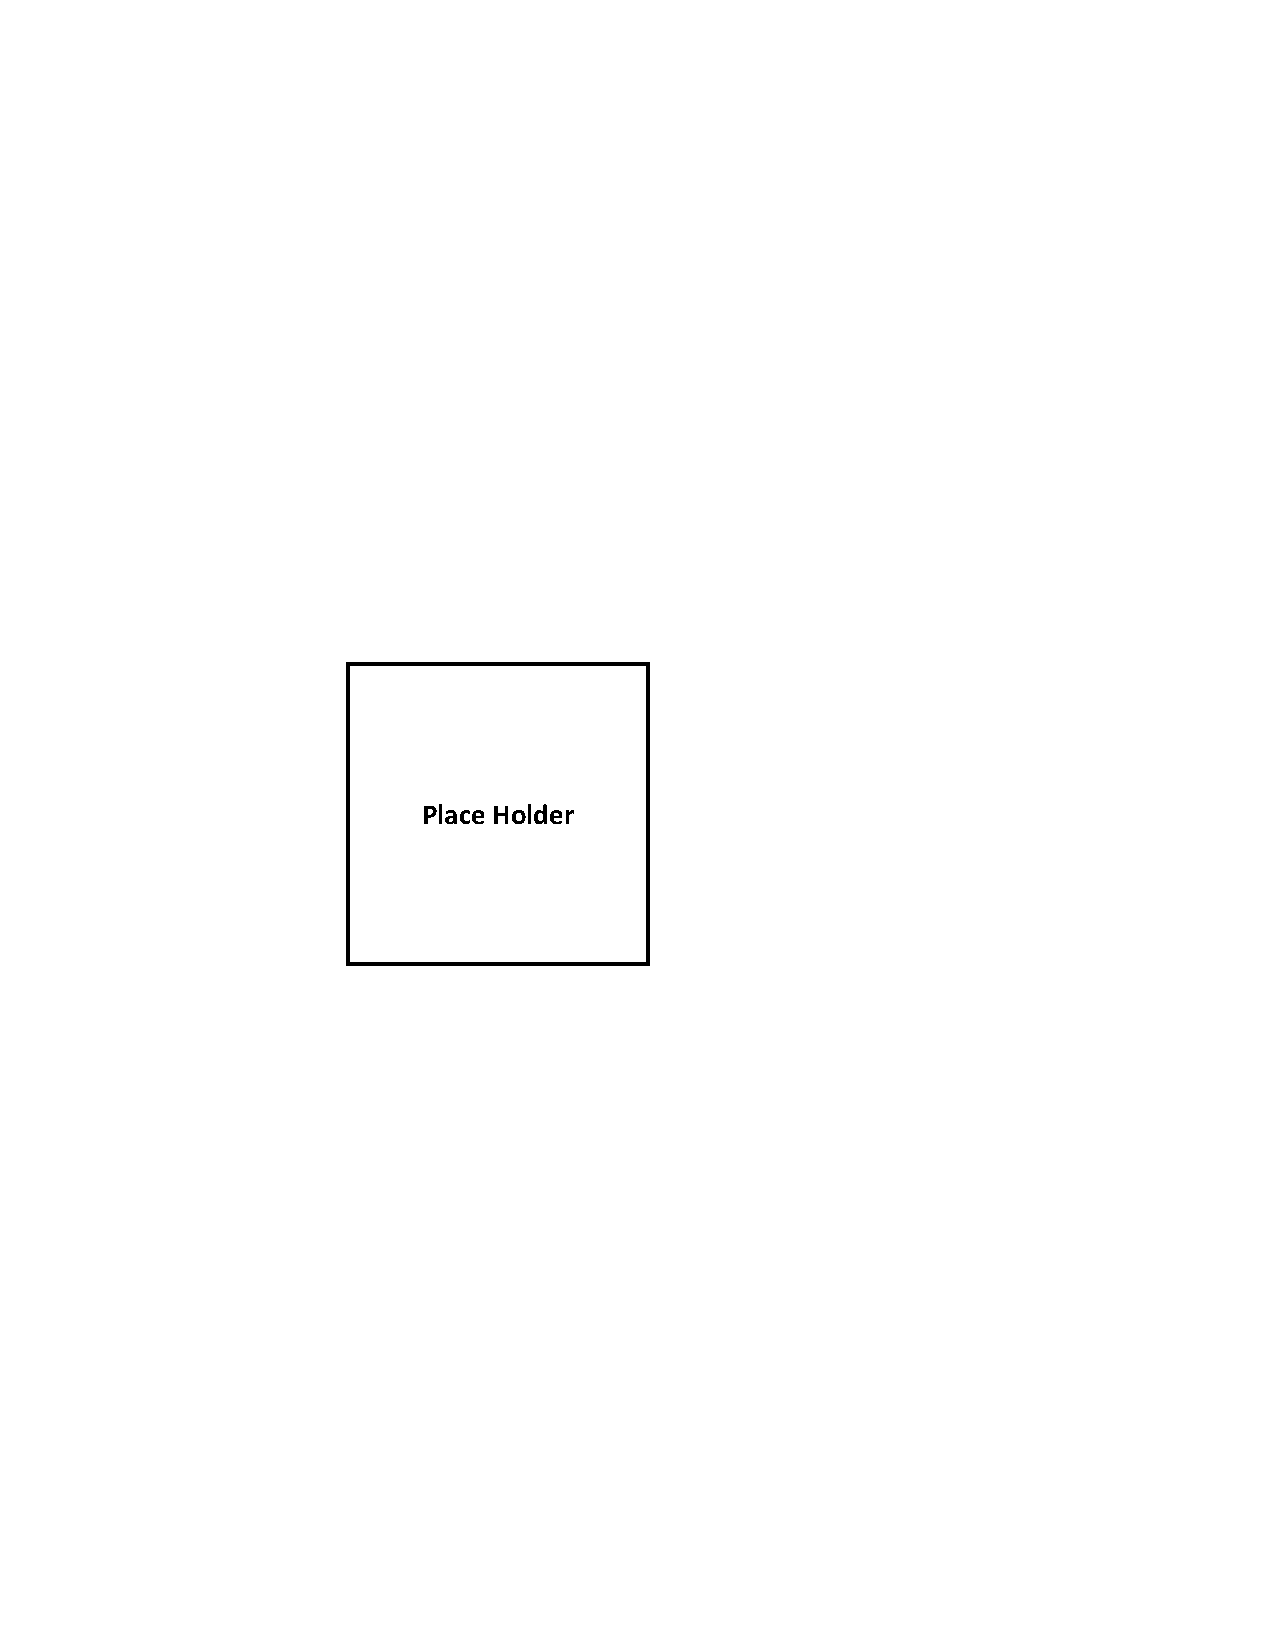
\includegraphics[width=\linewidth]{fig/PlaceHolder.pdf}
		\centerline{\dsali}
	\end{minipage}
	\hfill
	\begin{minipage}{0.18\linewidth}\centering
		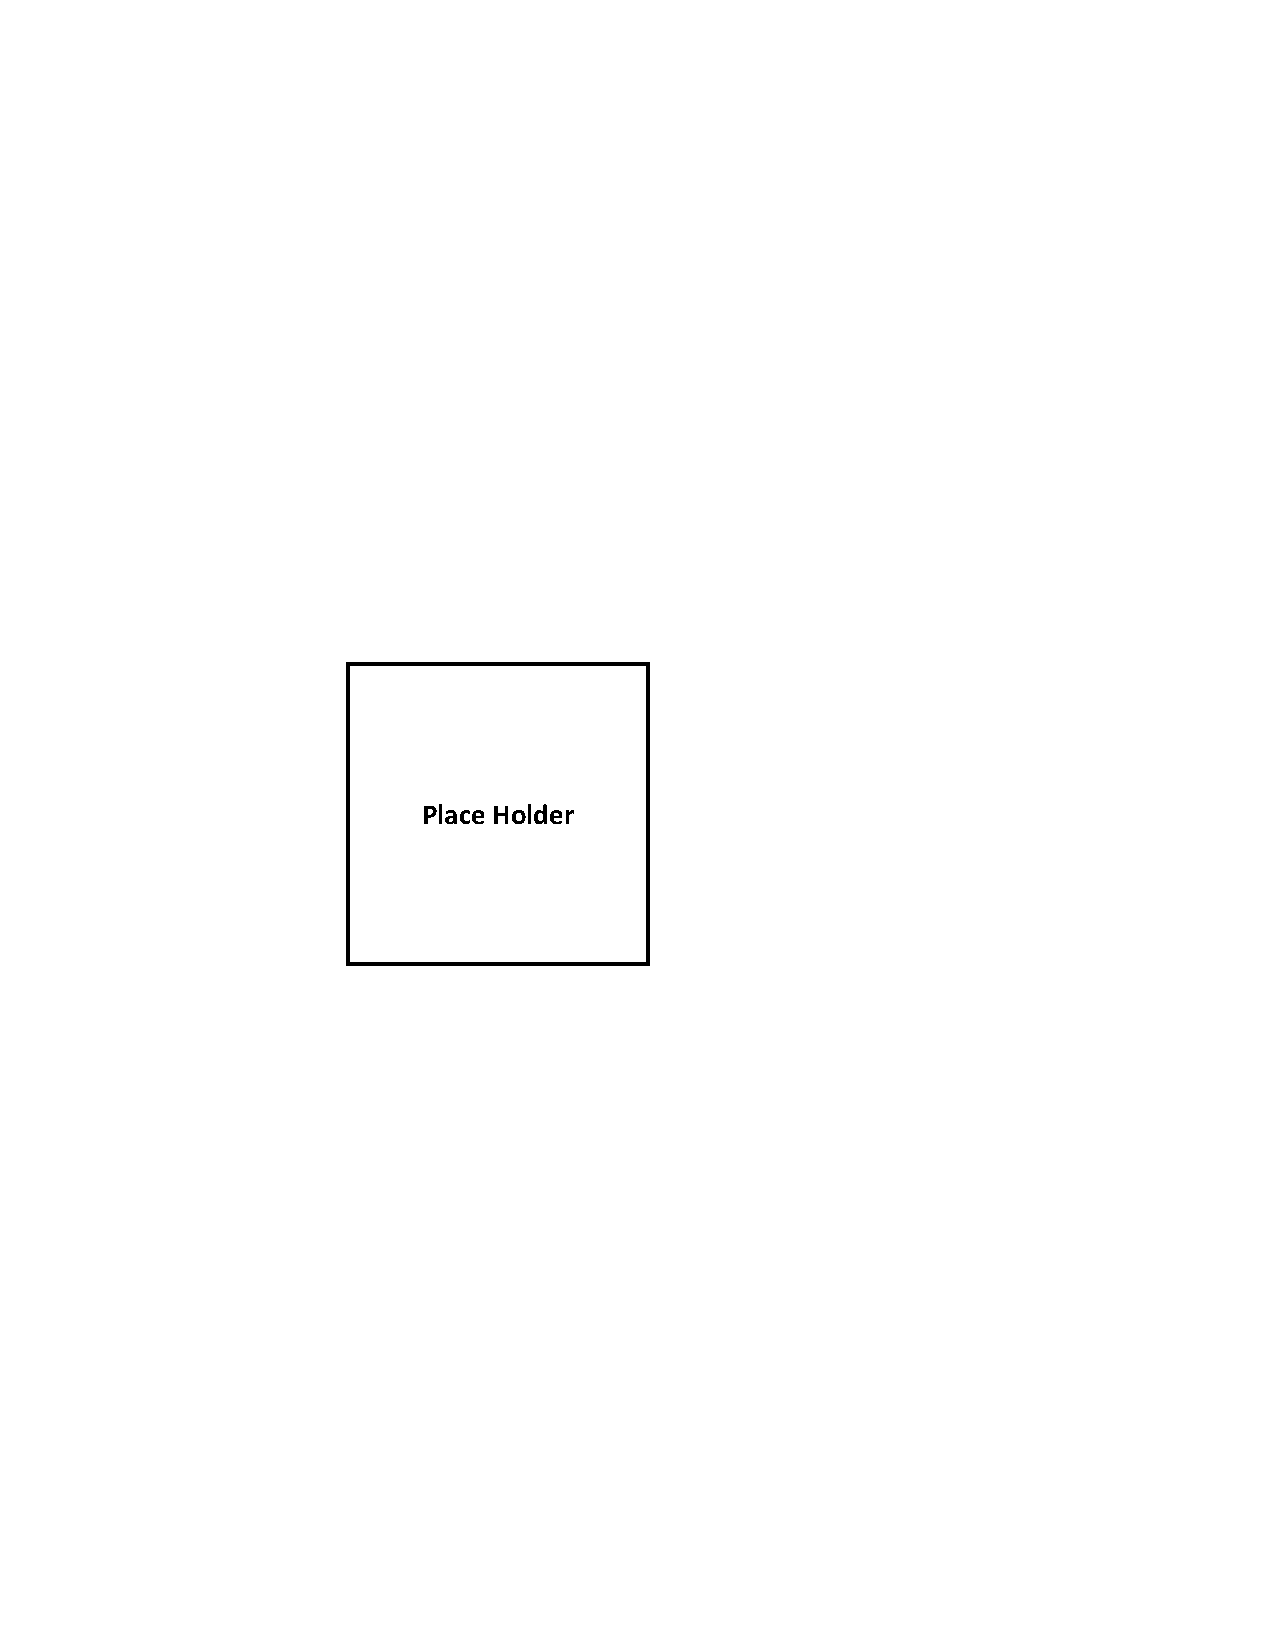
\includegraphics[width=\linewidth]{fig/PlaceHolder.pdf}
		\centerline{\dsrandom}
	\end{minipage}
	\caption{Run time for varying $\alpha$.}
	\label{fig:vary-alpha-time}
\end{figure*}

\begin{figure*}[h]
	\begin{minipage}{0.18\linewidth}\centering
		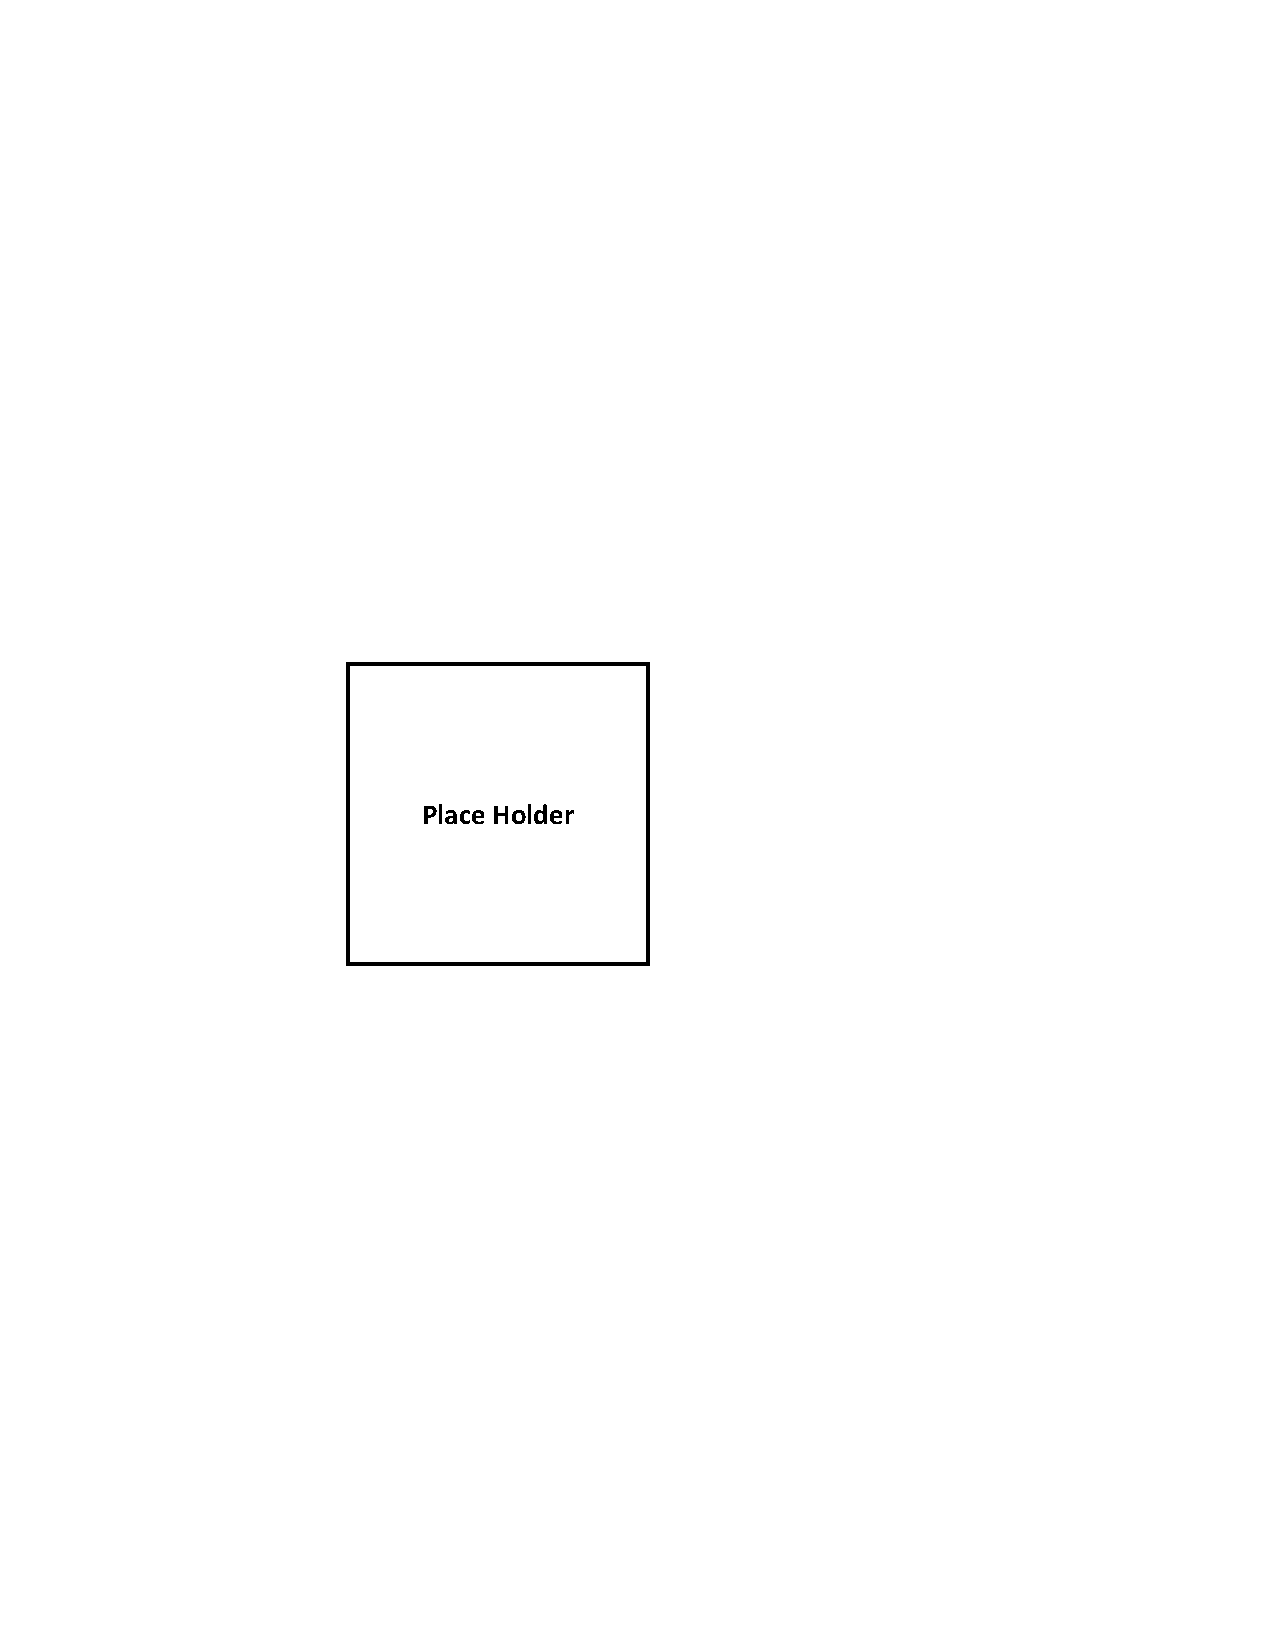
\includegraphics[width=\linewidth]{fig/PlaceHolder.pdf}
		\centerline{\dstwitter}
	\end{minipage}
	\hfill
	\begin{minipage}{0.18\linewidth}\centering
		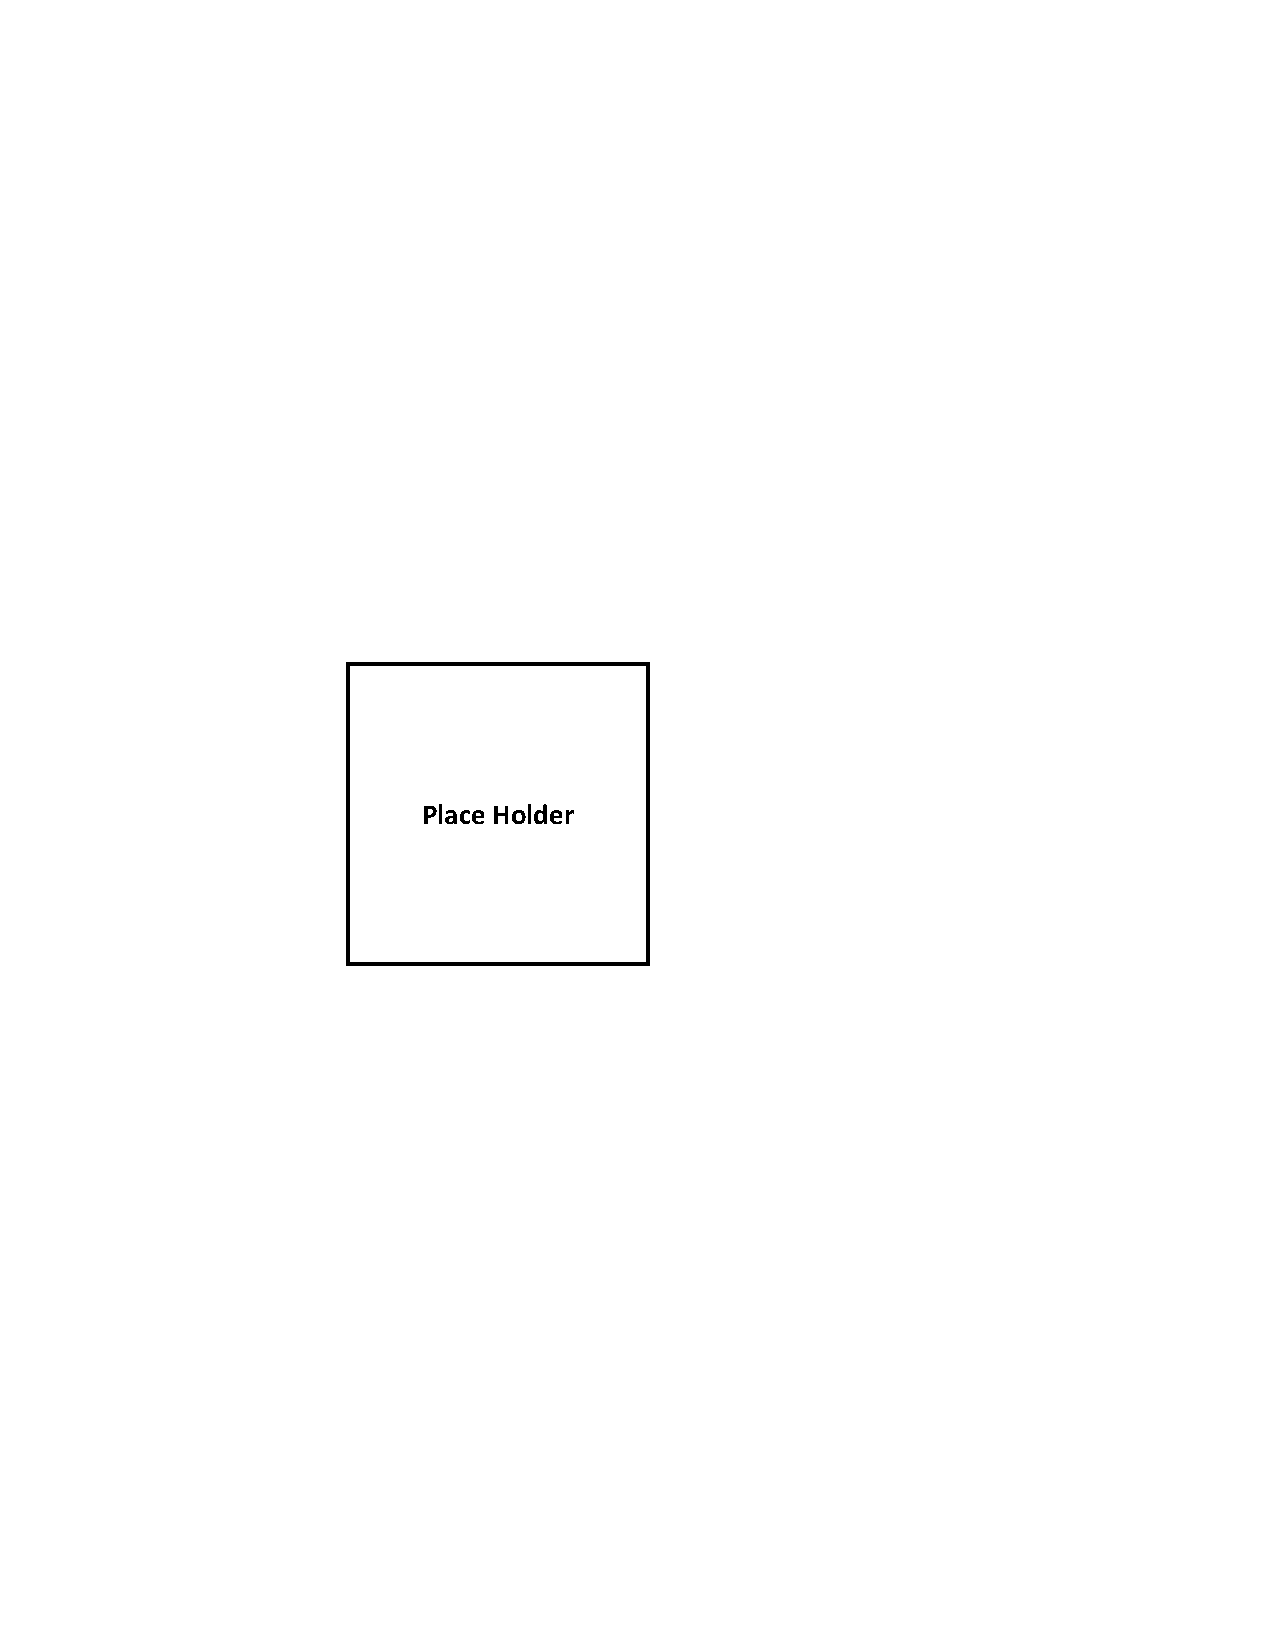
\includegraphics[width=\linewidth]{fig/PlaceHolder.pdf}
		\centerline{\dsreddit}
	\end{minipage}
	\hfill
	\begin{minipage}{0.18\linewidth}\centering
		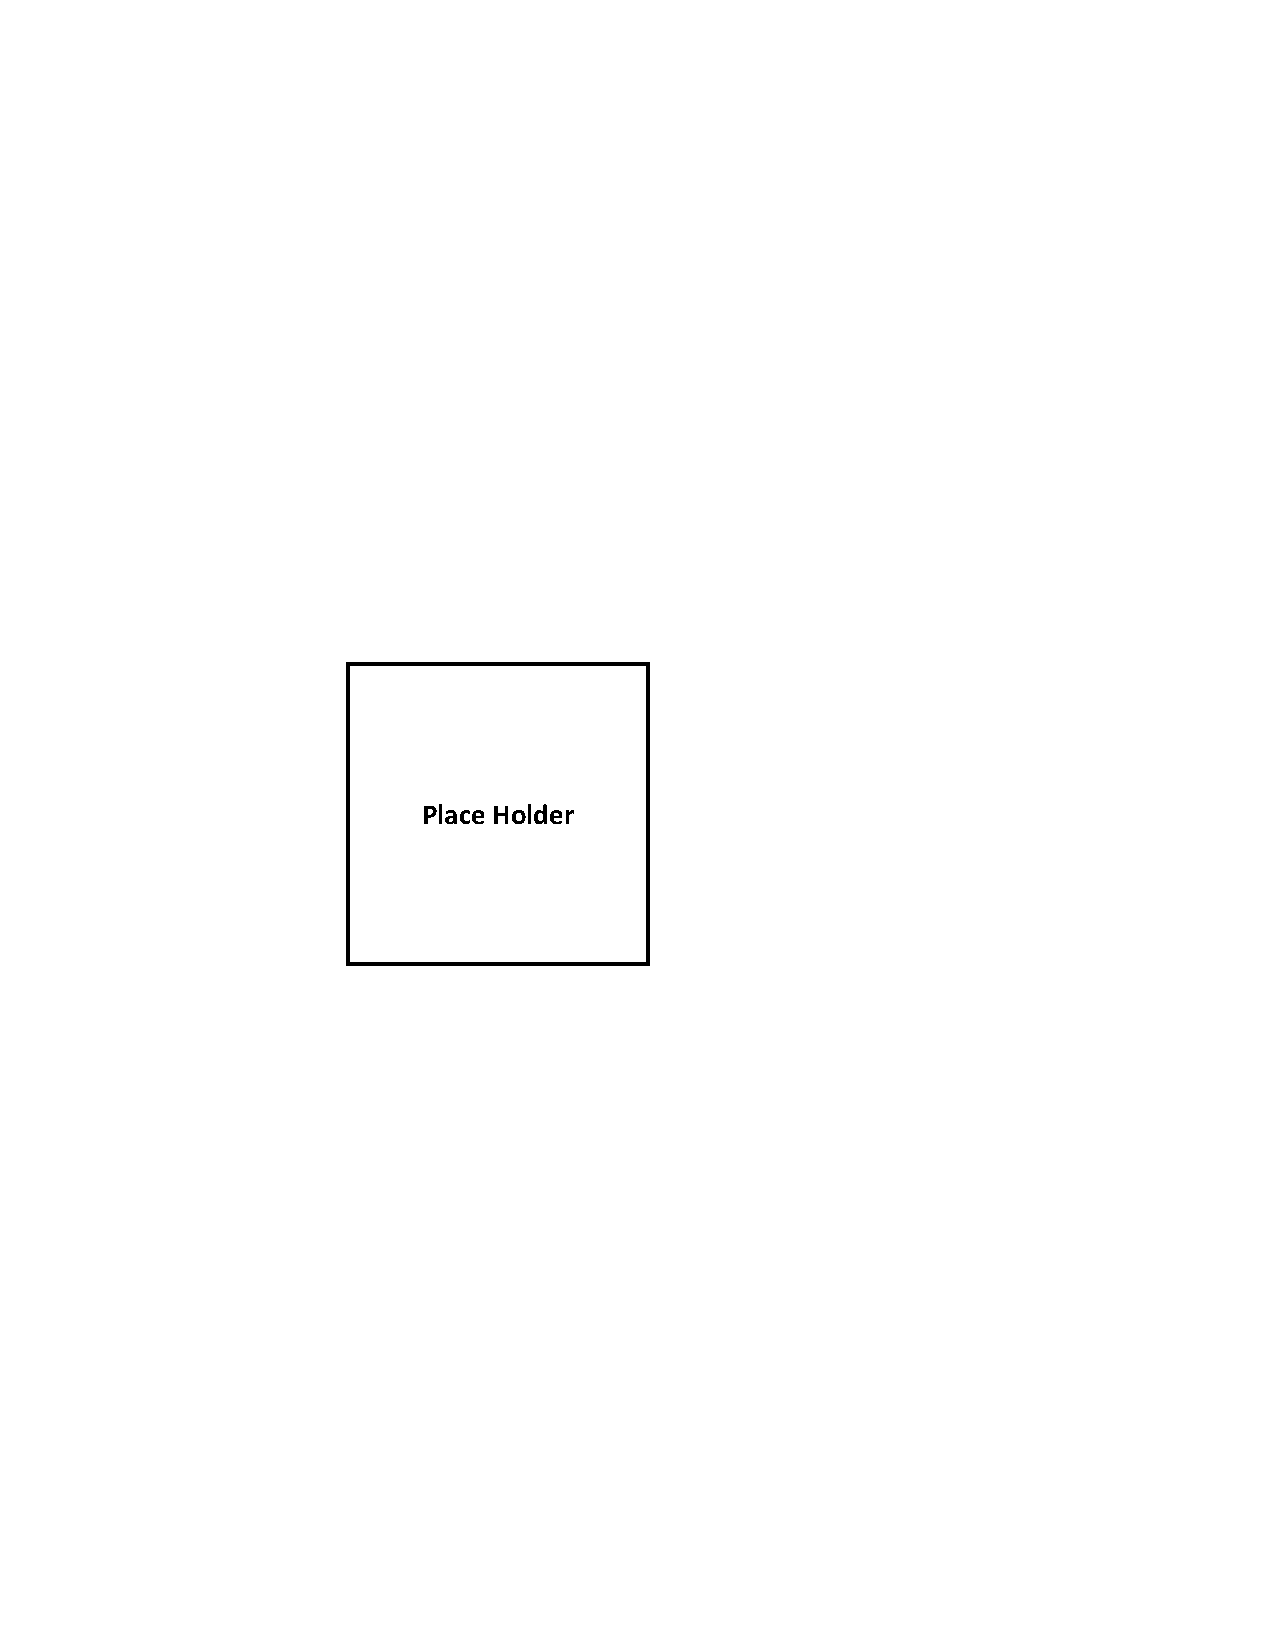
\includegraphics[width=\linewidth]{fig/PlaceHolder.pdf}
		\centerline{\dstpch}
	\end{minipage}
	\hfill
	\begin{minipage}{0.18\linewidth}\centering
		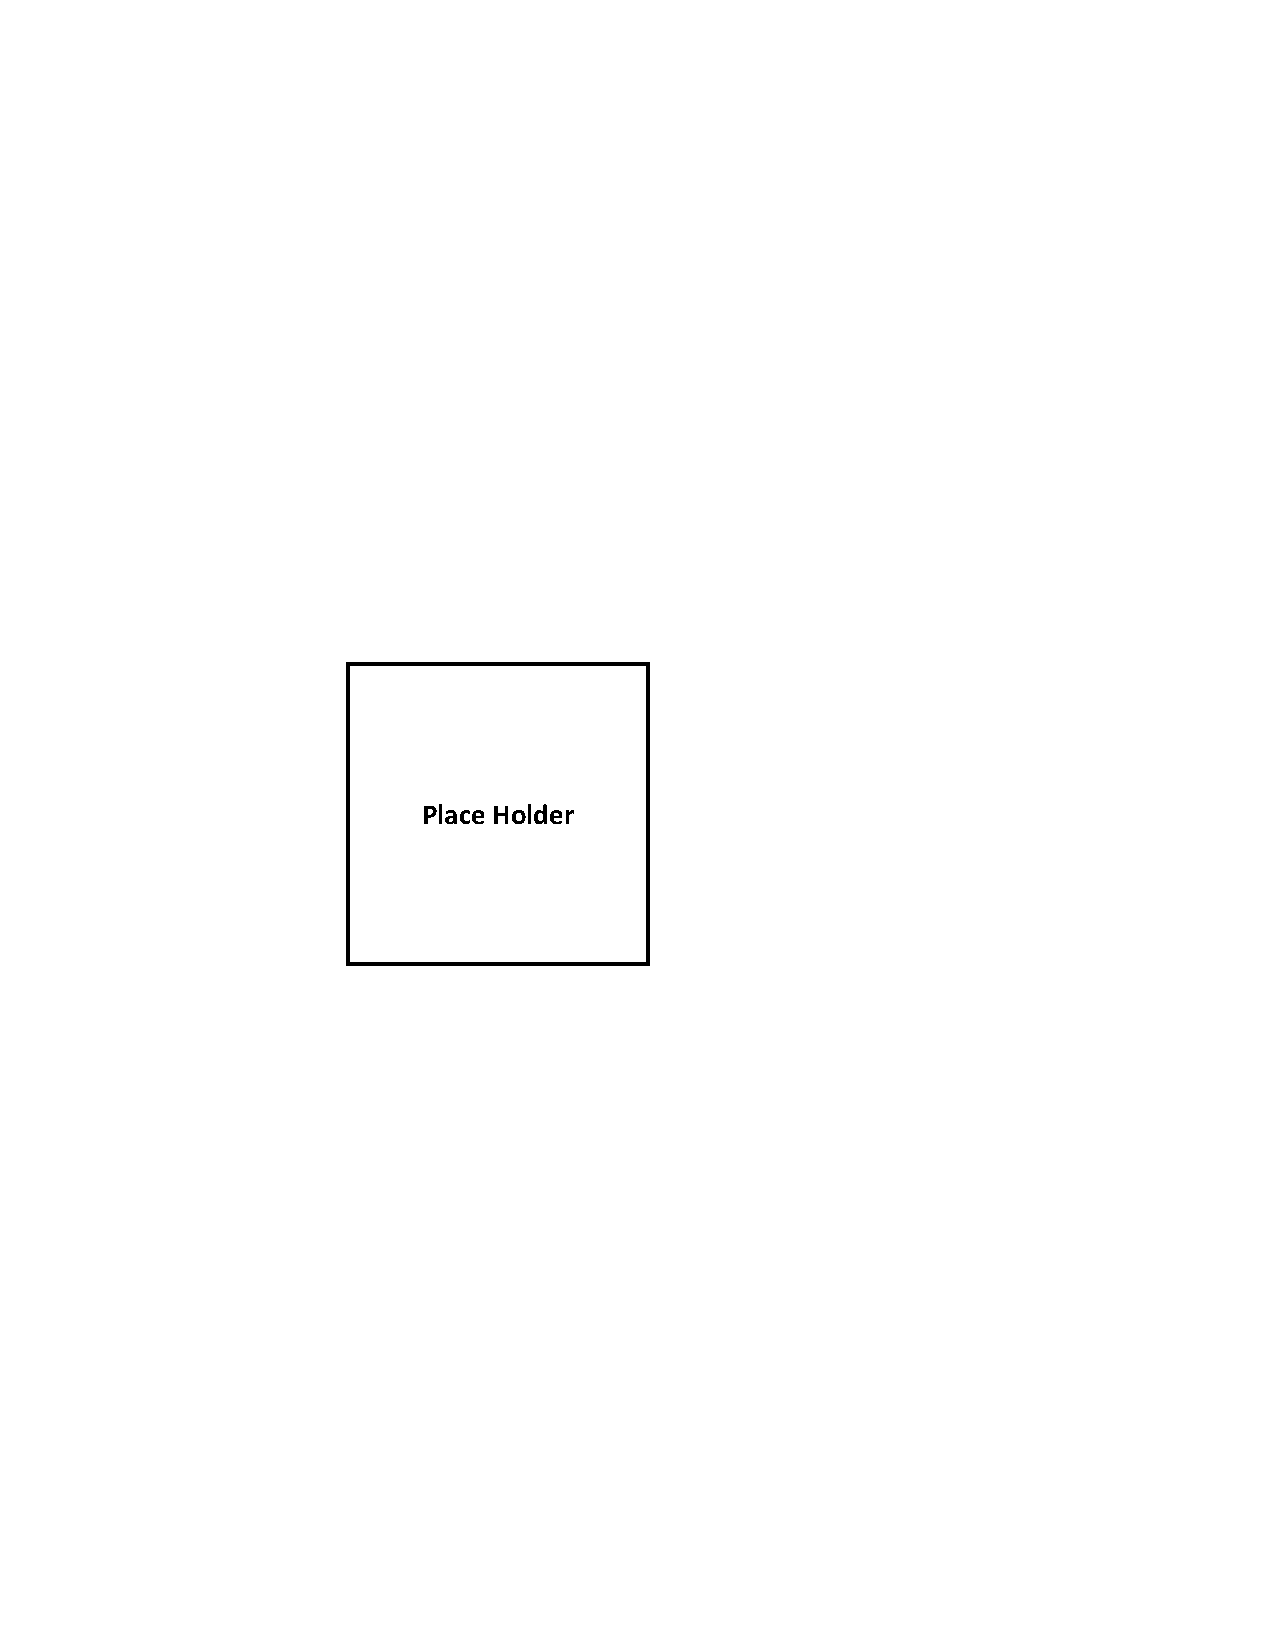
\includegraphics[width=\linewidth]{fig/PlaceHolder.pdf}
		\centerline{\dsali}
	\end{minipage}
	\hfill
	\begin{minipage}{0.18\linewidth}\centering
		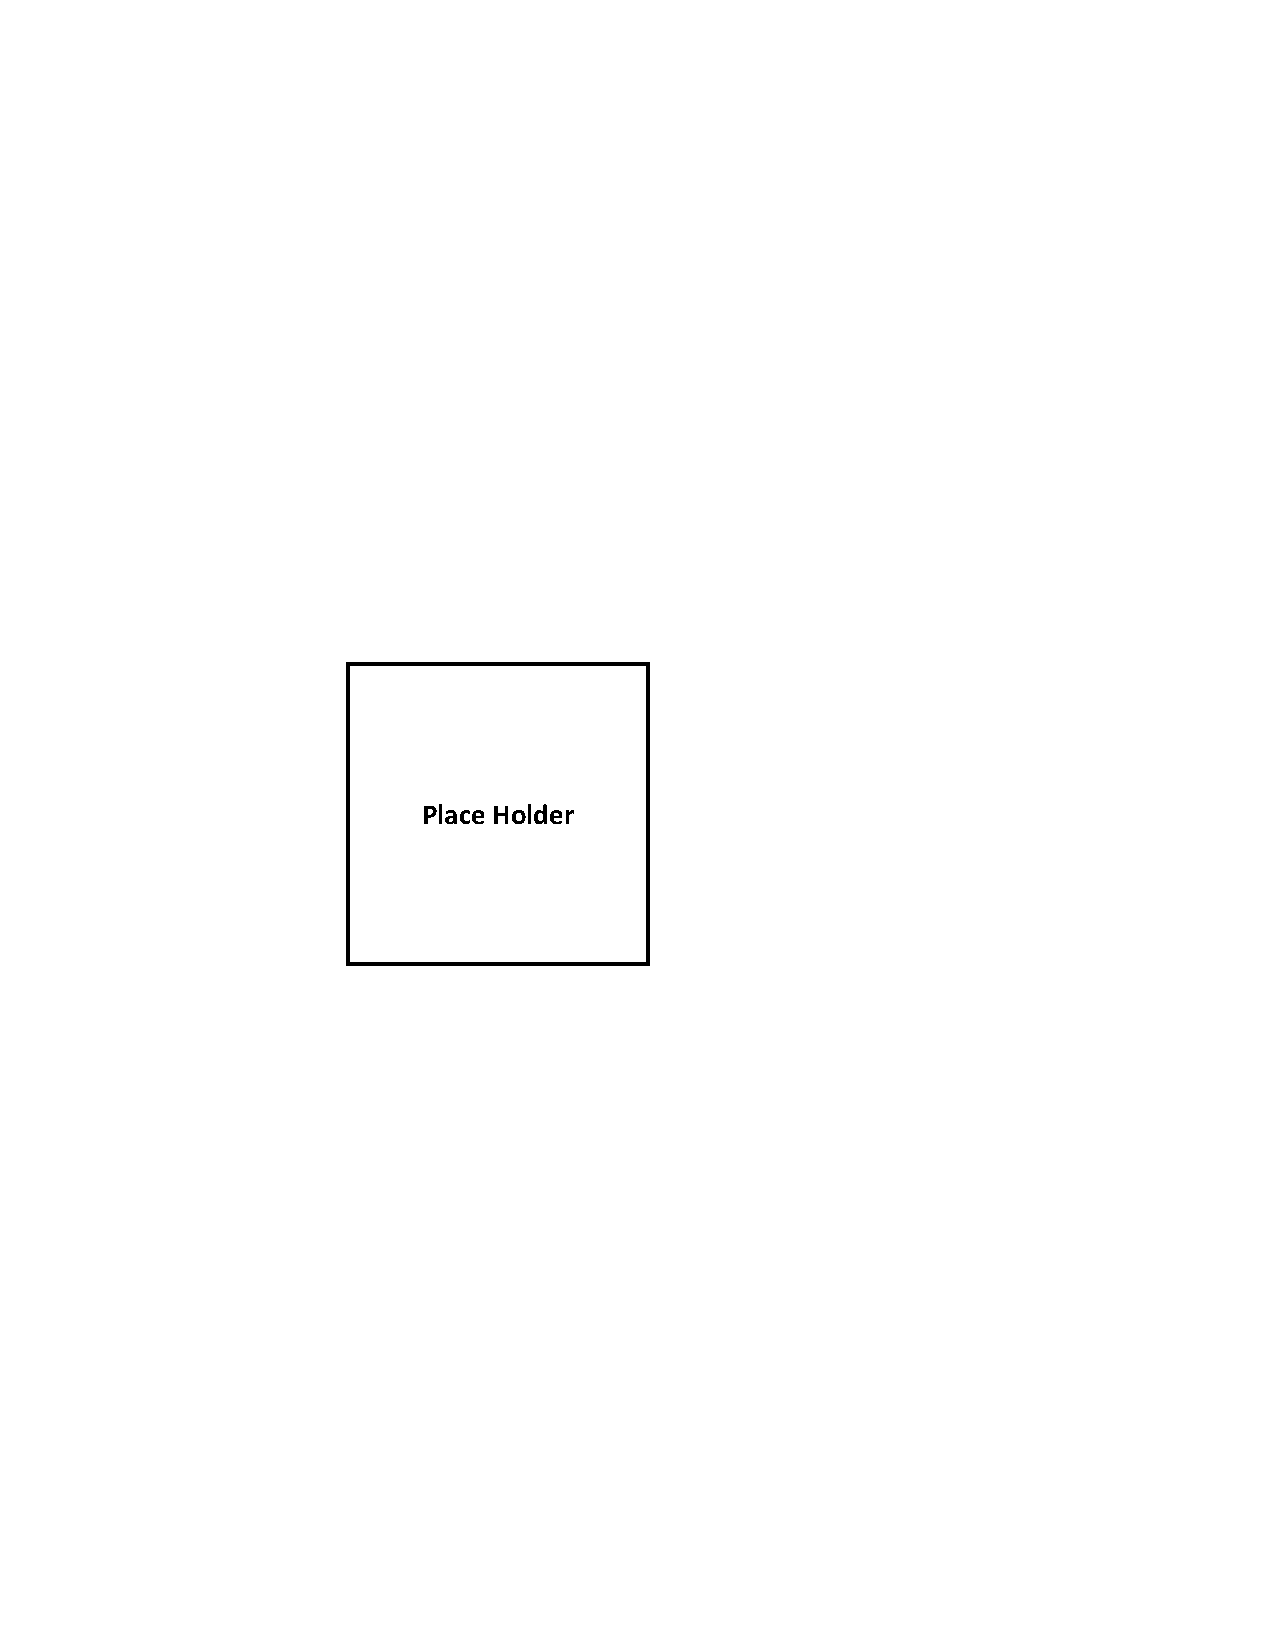
\includegraphics[width=\linewidth]{fig/PlaceHolder.pdf}
		\centerline{\dsrandom}
	\end{minipage}
	\caption{System stability for varying $\alpha$.}
	\label{fig:vary-alpha-stability}
\end{figure*}

\vspace{1mm}\noindent\textbf{Varying the filled factor upper bound $\beta$.}

\begin{figure*}[h]
	\begin{minipage}{0.18\linewidth}\centering
		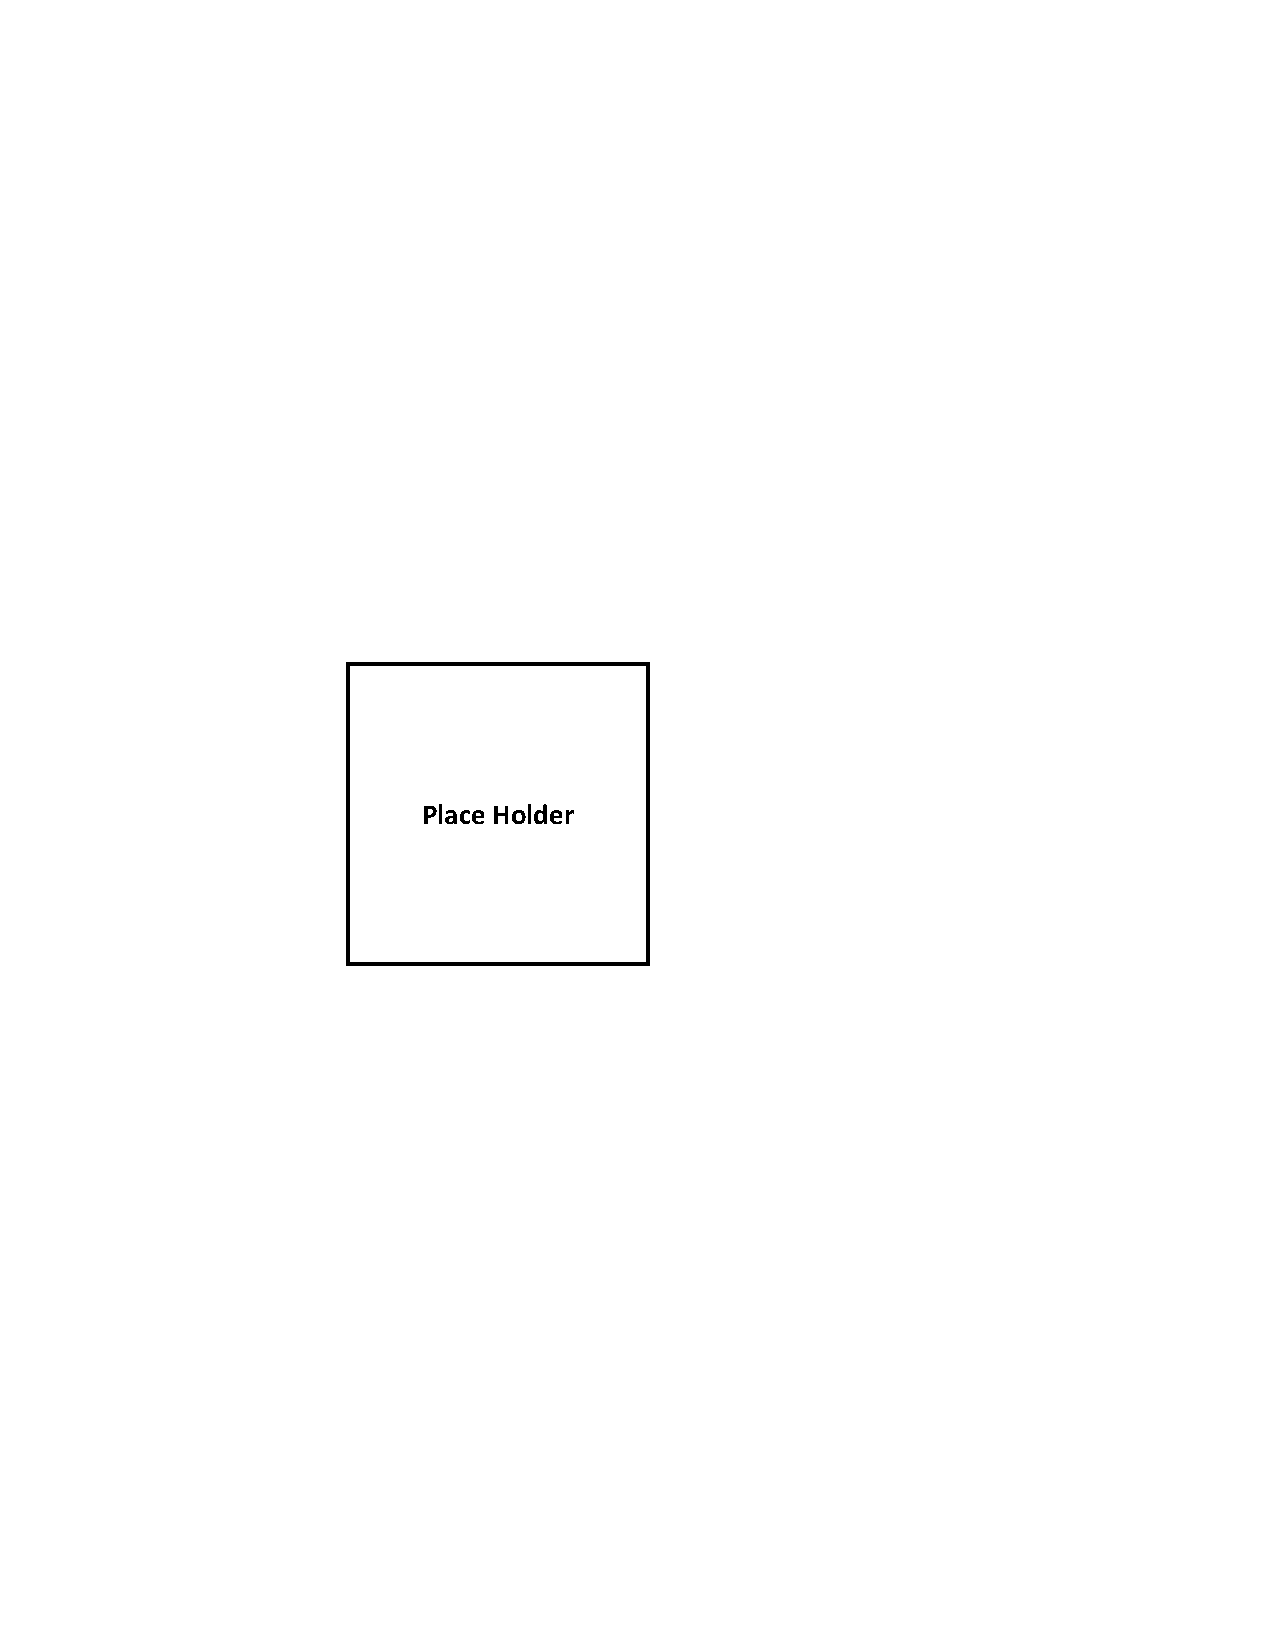
\includegraphics[width=\linewidth]{fig/PlaceHolder.pdf}
		\centerline{\dstwitter}
	\end{minipage}
	\hfill
	\begin{minipage}{0.18\linewidth}\centering
		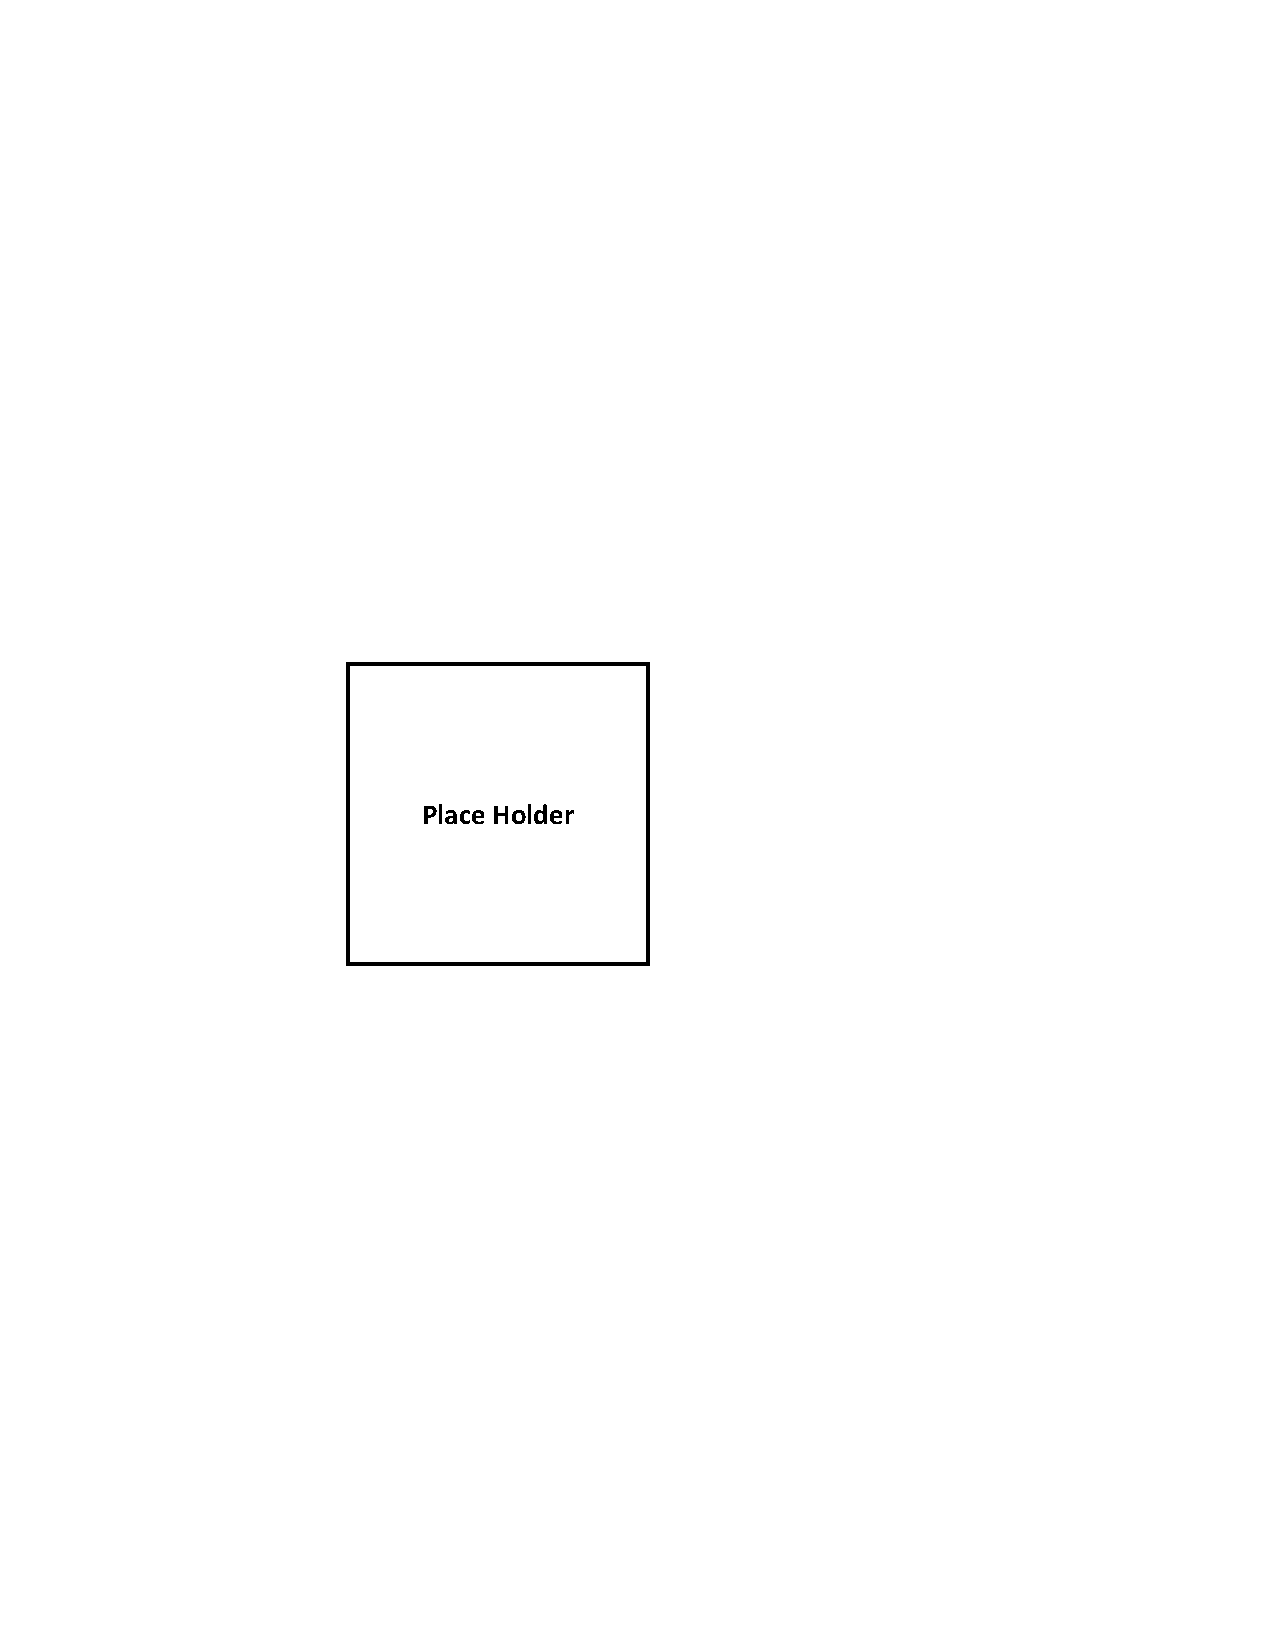
\includegraphics[width=\linewidth]{fig/PlaceHolder.pdf}
		\centerline{\dsreddit}
	\end{minipage}
	\hfill
	\begin{minipage}{0.18\linewidth}\centering
		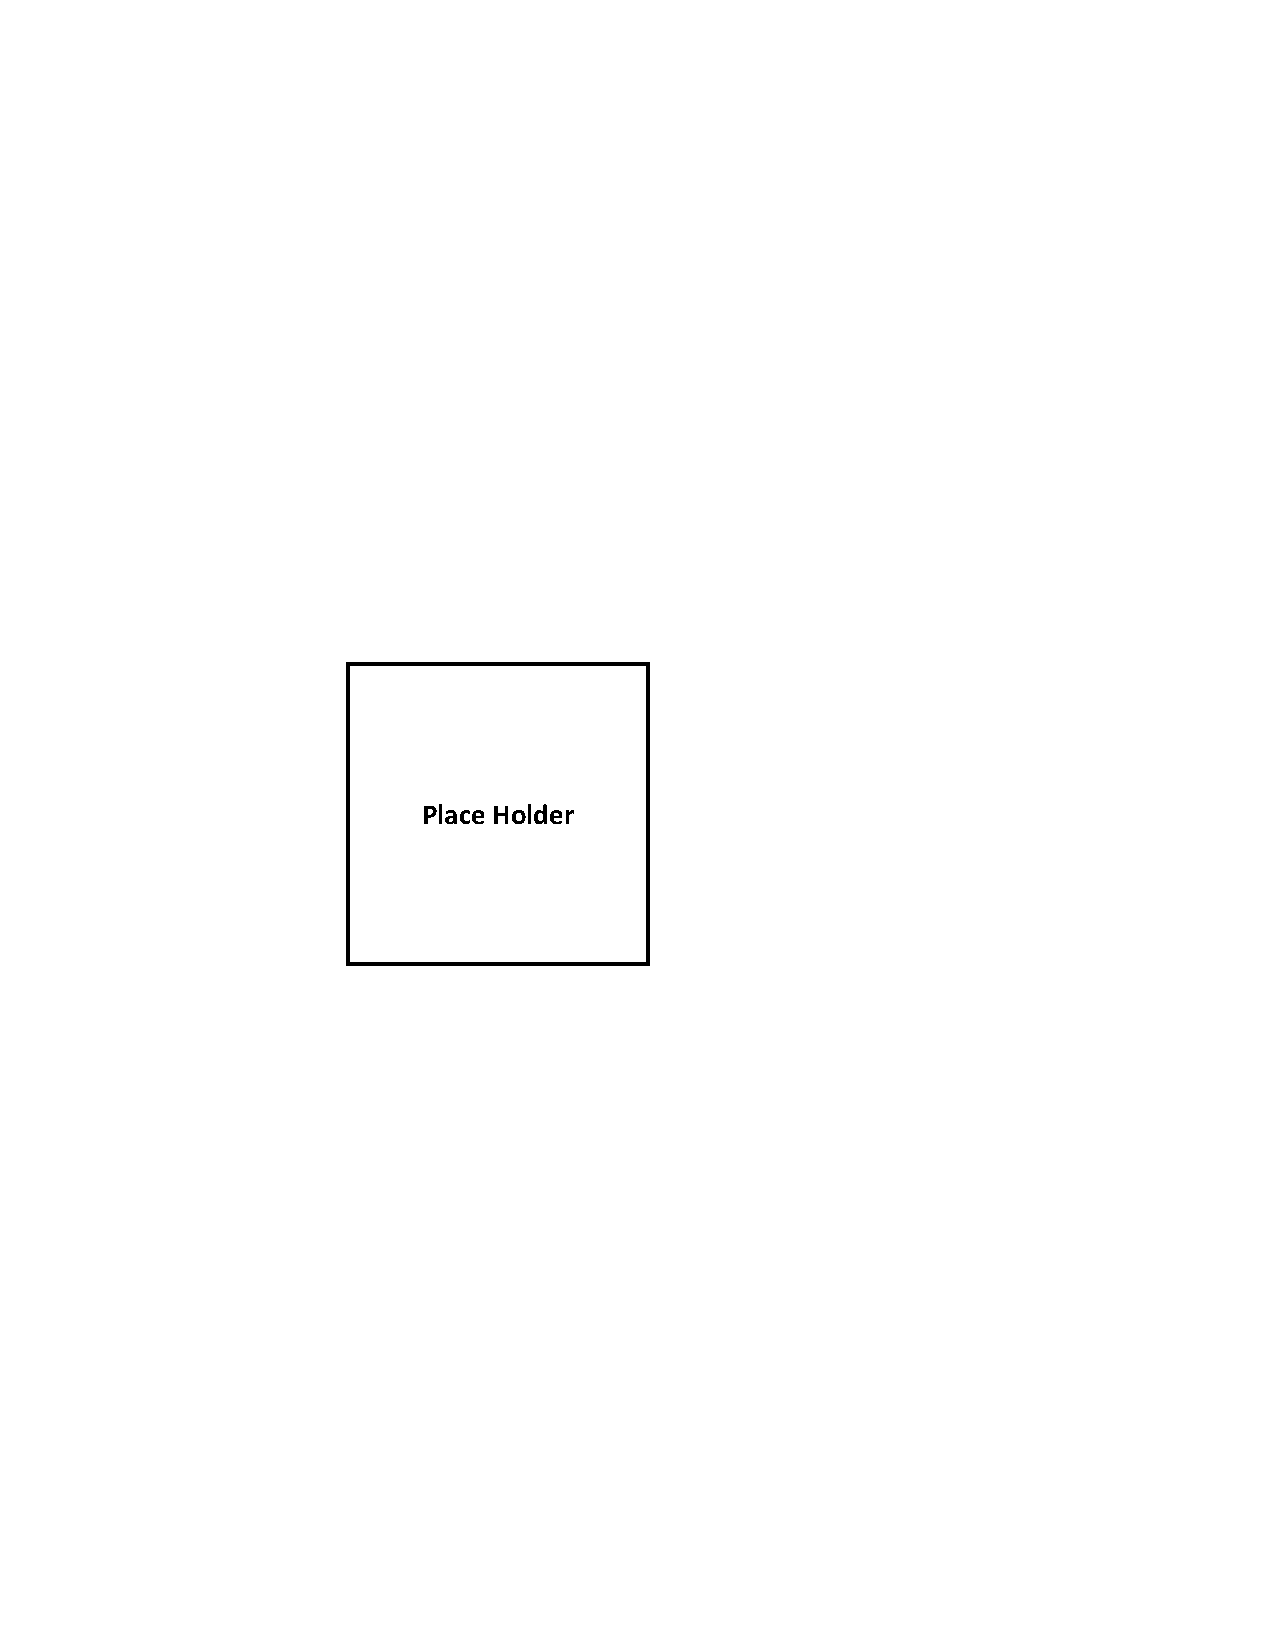
\includegraphics[width=\linewidth]{fig/PlaceHolder.pdf}
		\centerline{\dstpch}
	\end{minipage}
	\hfill
	\begin{minipage}{0.18\linewidth}\centering
		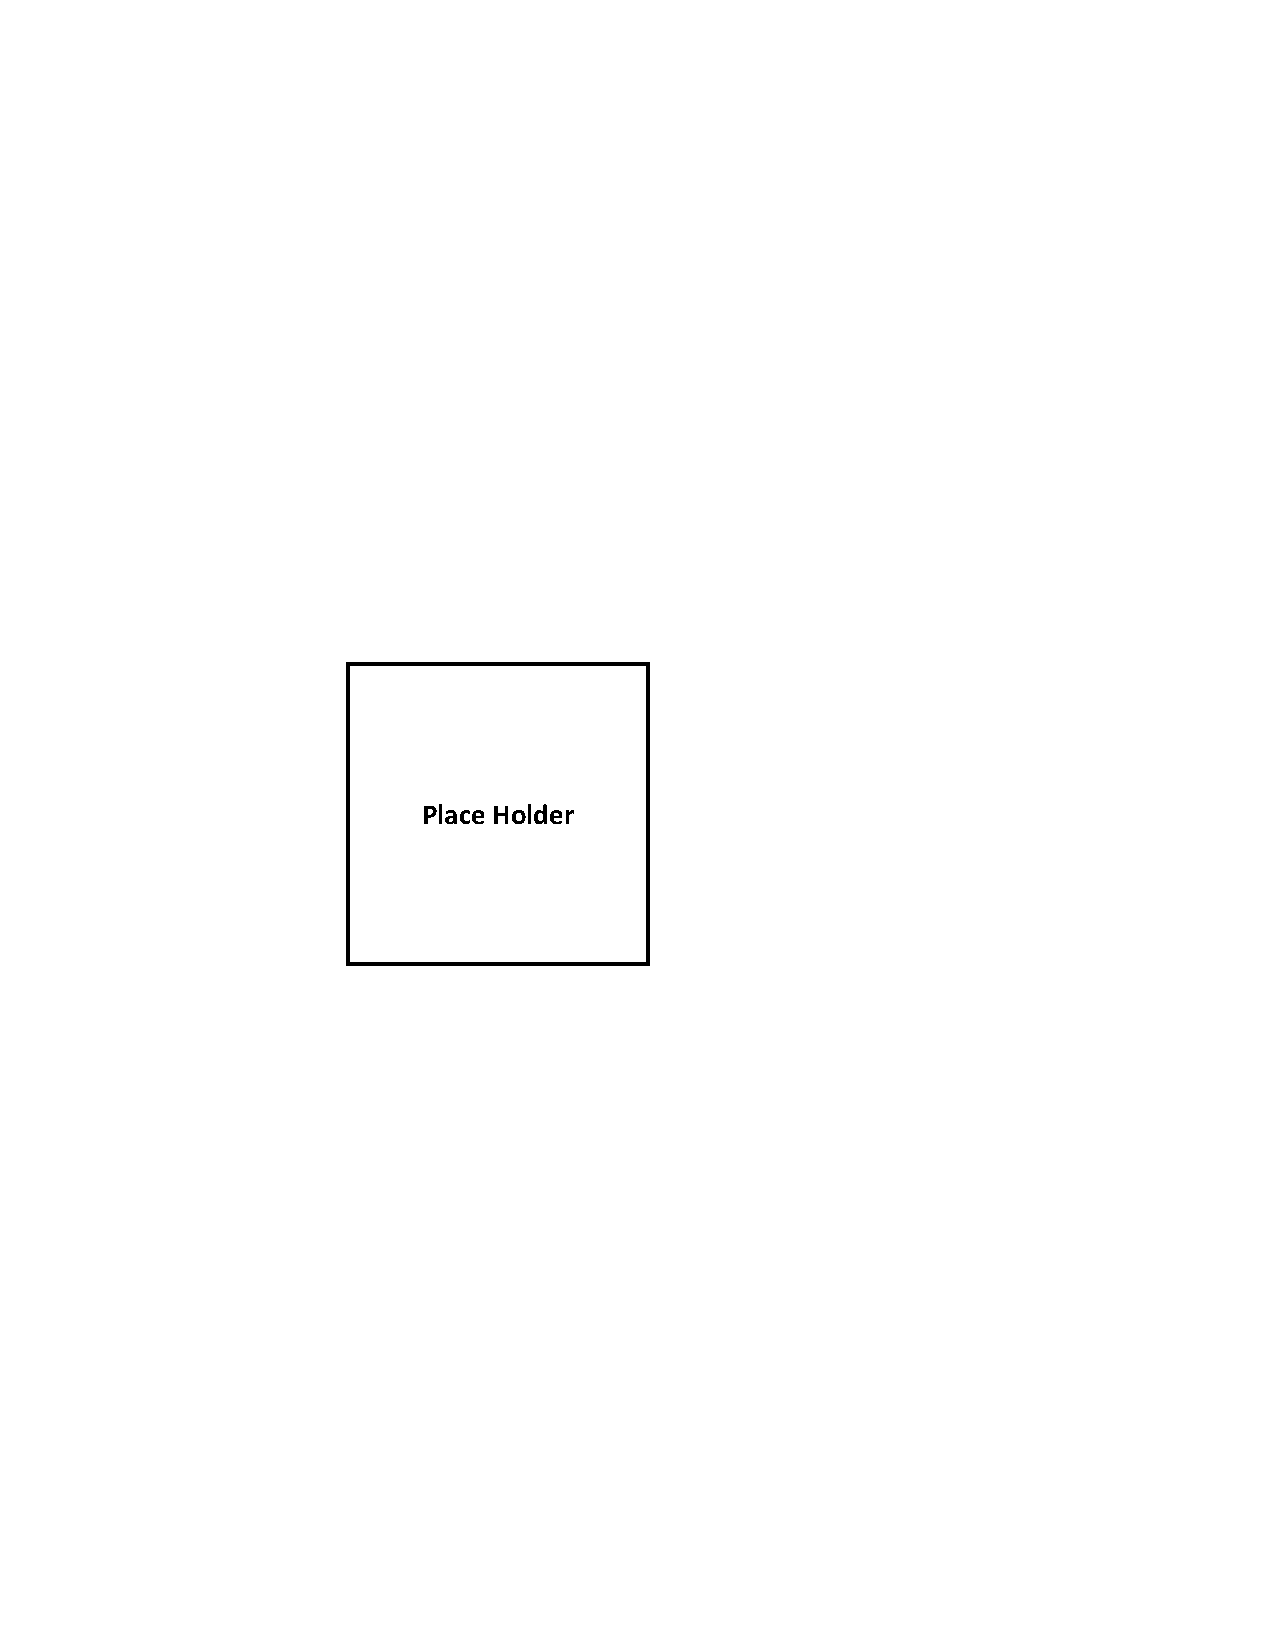
\includegraphics[width=\linewidth]{fig/PlaceHolder.pdf}
		\centerline{\dsali}
	\end{minipage}
	\hfill
	\begin{minipage}{0.18\linewidth}\centering
		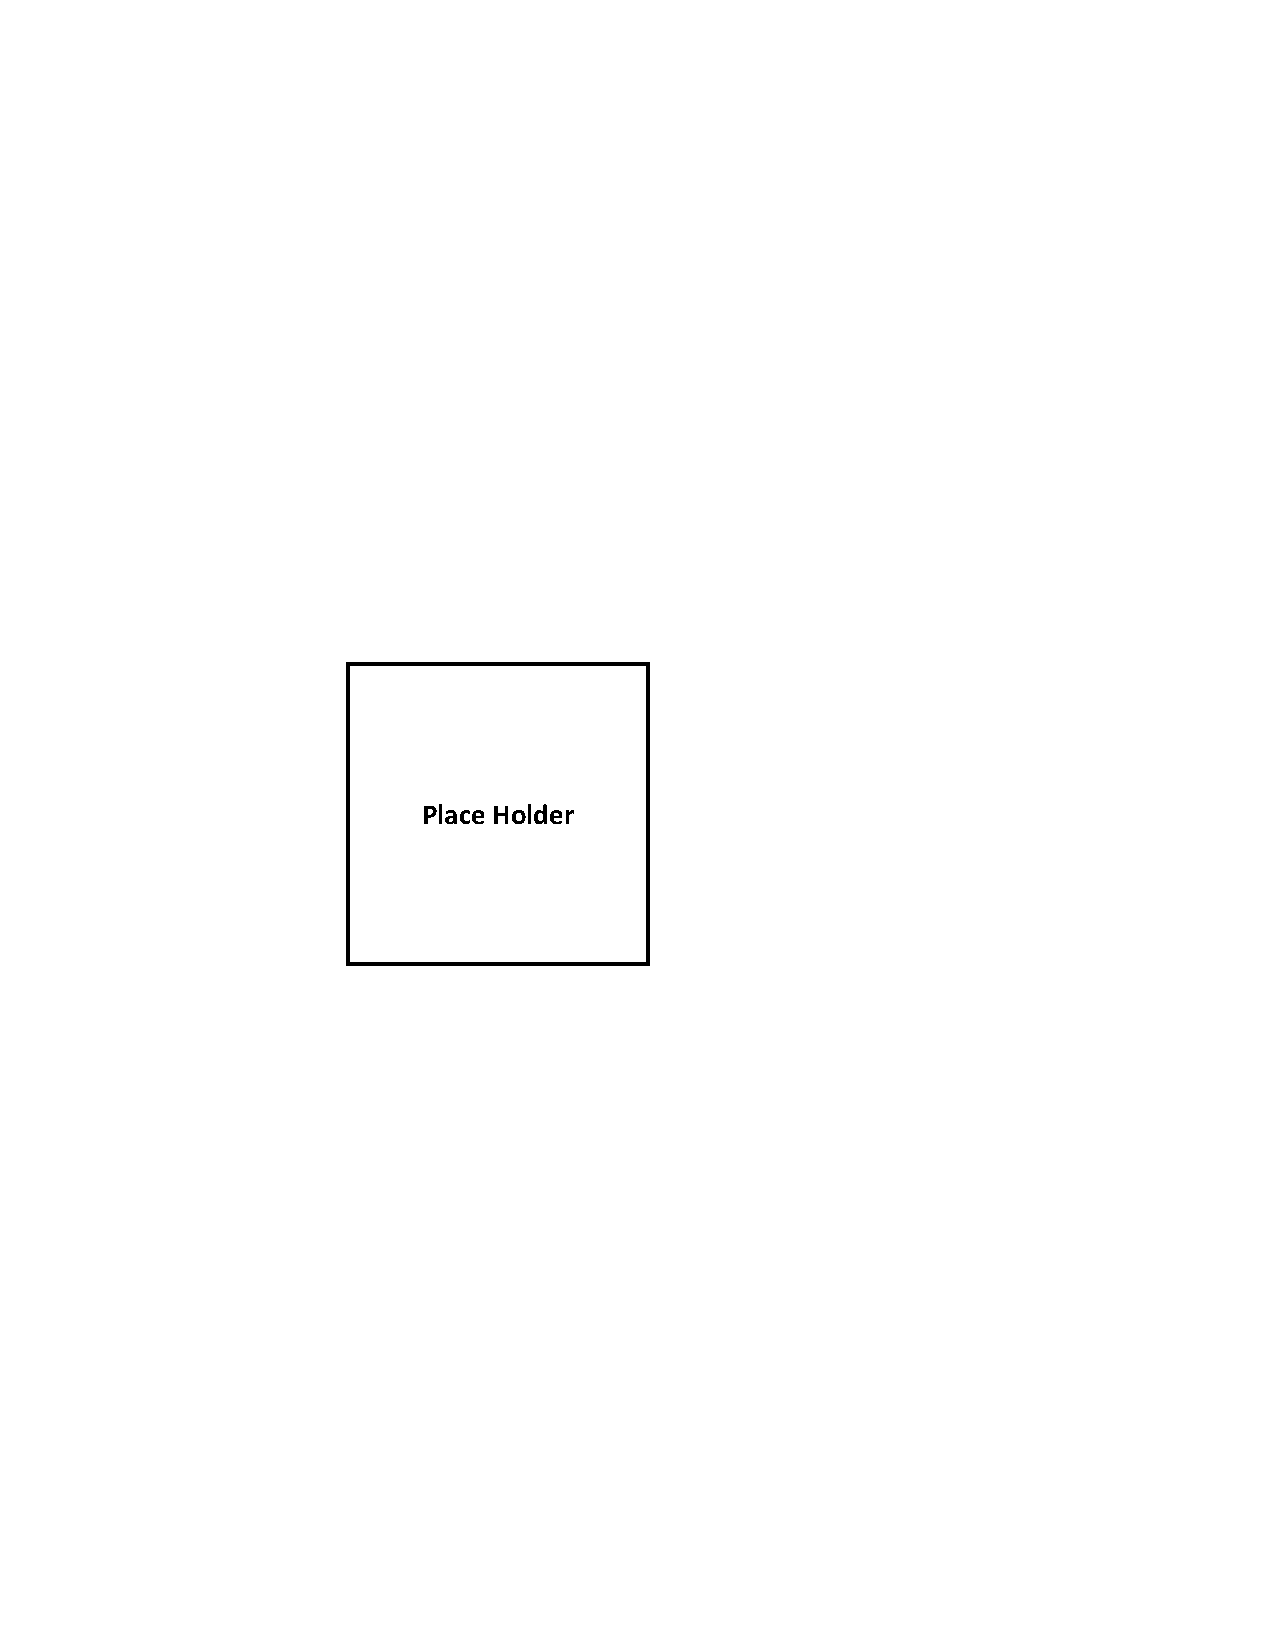
\includegraphics[width=\linewidth]{fig/PlaceHolder.pdf}
		\centerline{\dsrandom}
	\end{minipage}
	\caption{Run time for varying $\beta$.}
	\label{fig:vary-beta-time}
\end{figure*}

\vspace{1mm}\noindent\textbf{Varying insert vs. delete ratio $r$.}

\begin{figure*}[h]
	\begin{minipage}{0.18\linewidth}\centering
		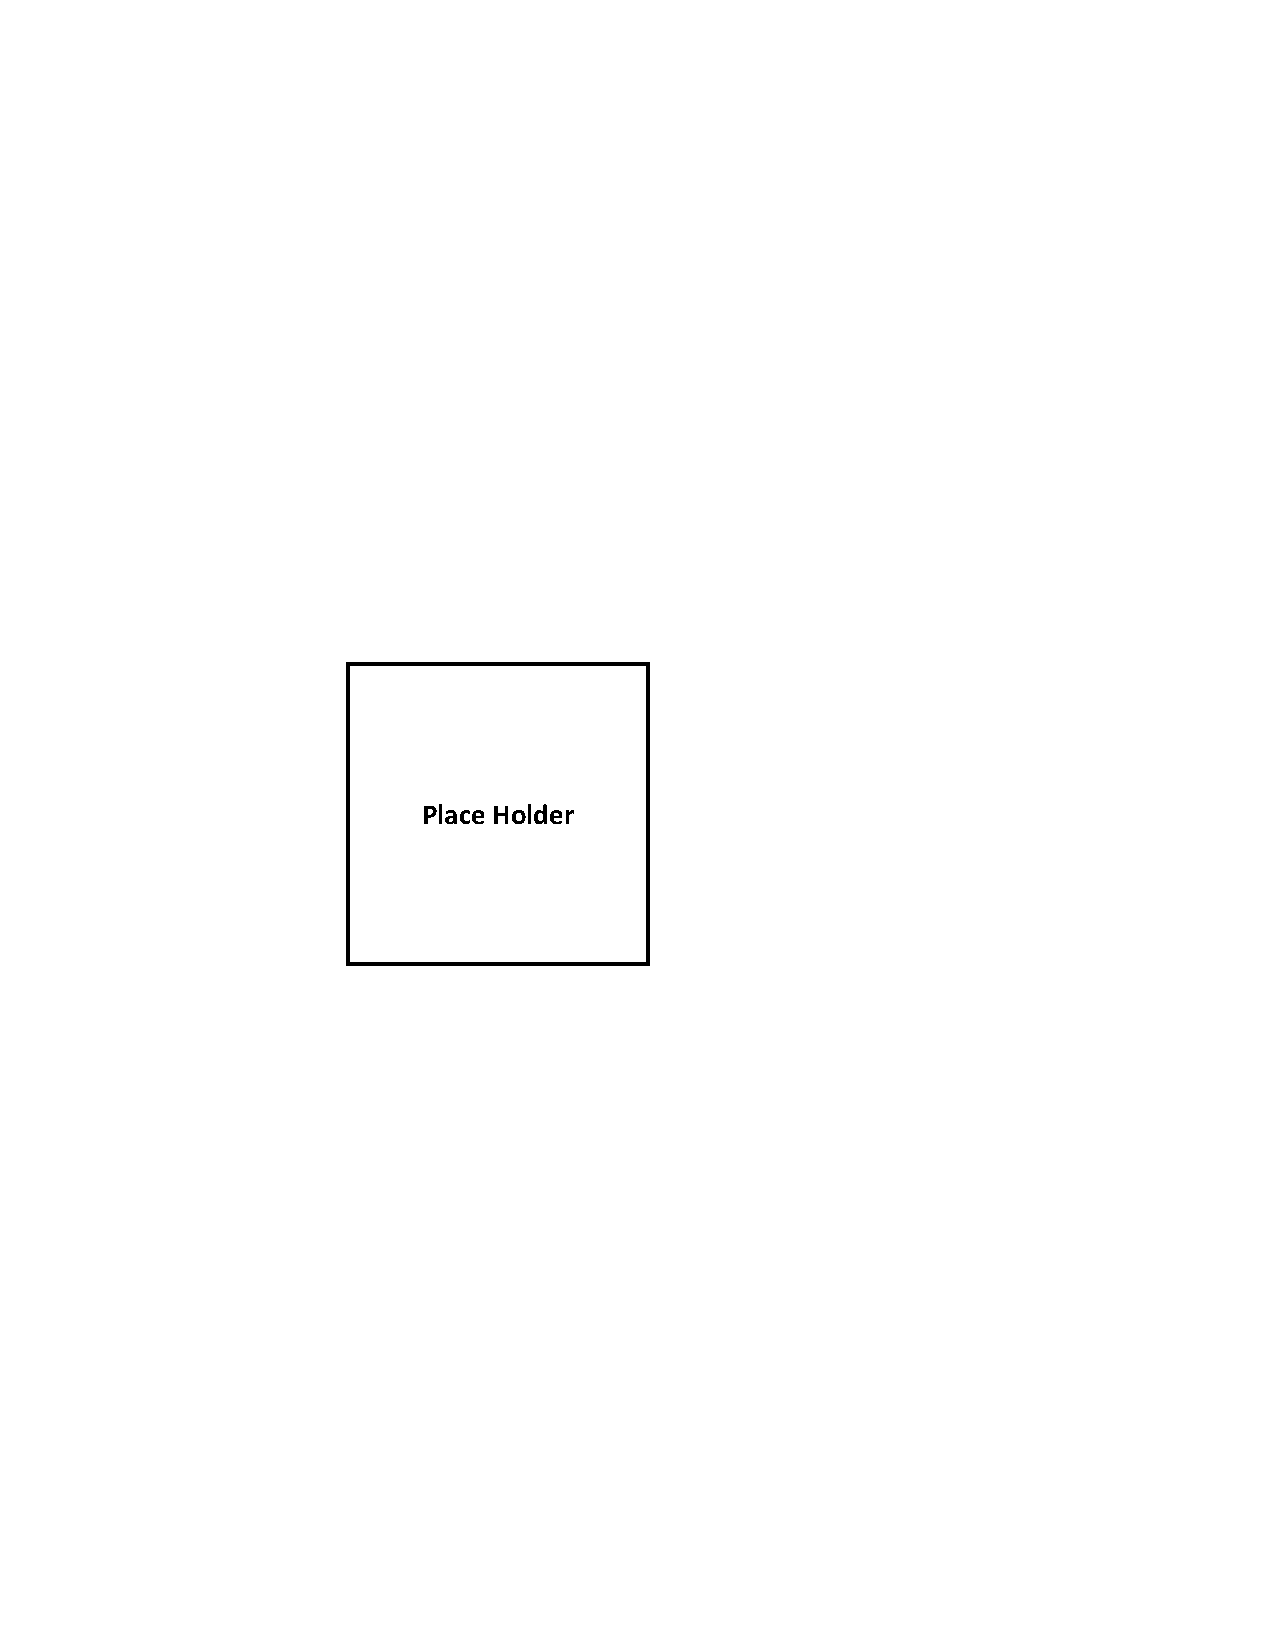
\includegraphics[width=\linewidth]{fig/PlaceHolder.pdf}
		\centerline{\dstwitter}
	\end{minipage}
	\hfill
	\begin{minipage}{0.18\linewidth}\centering
		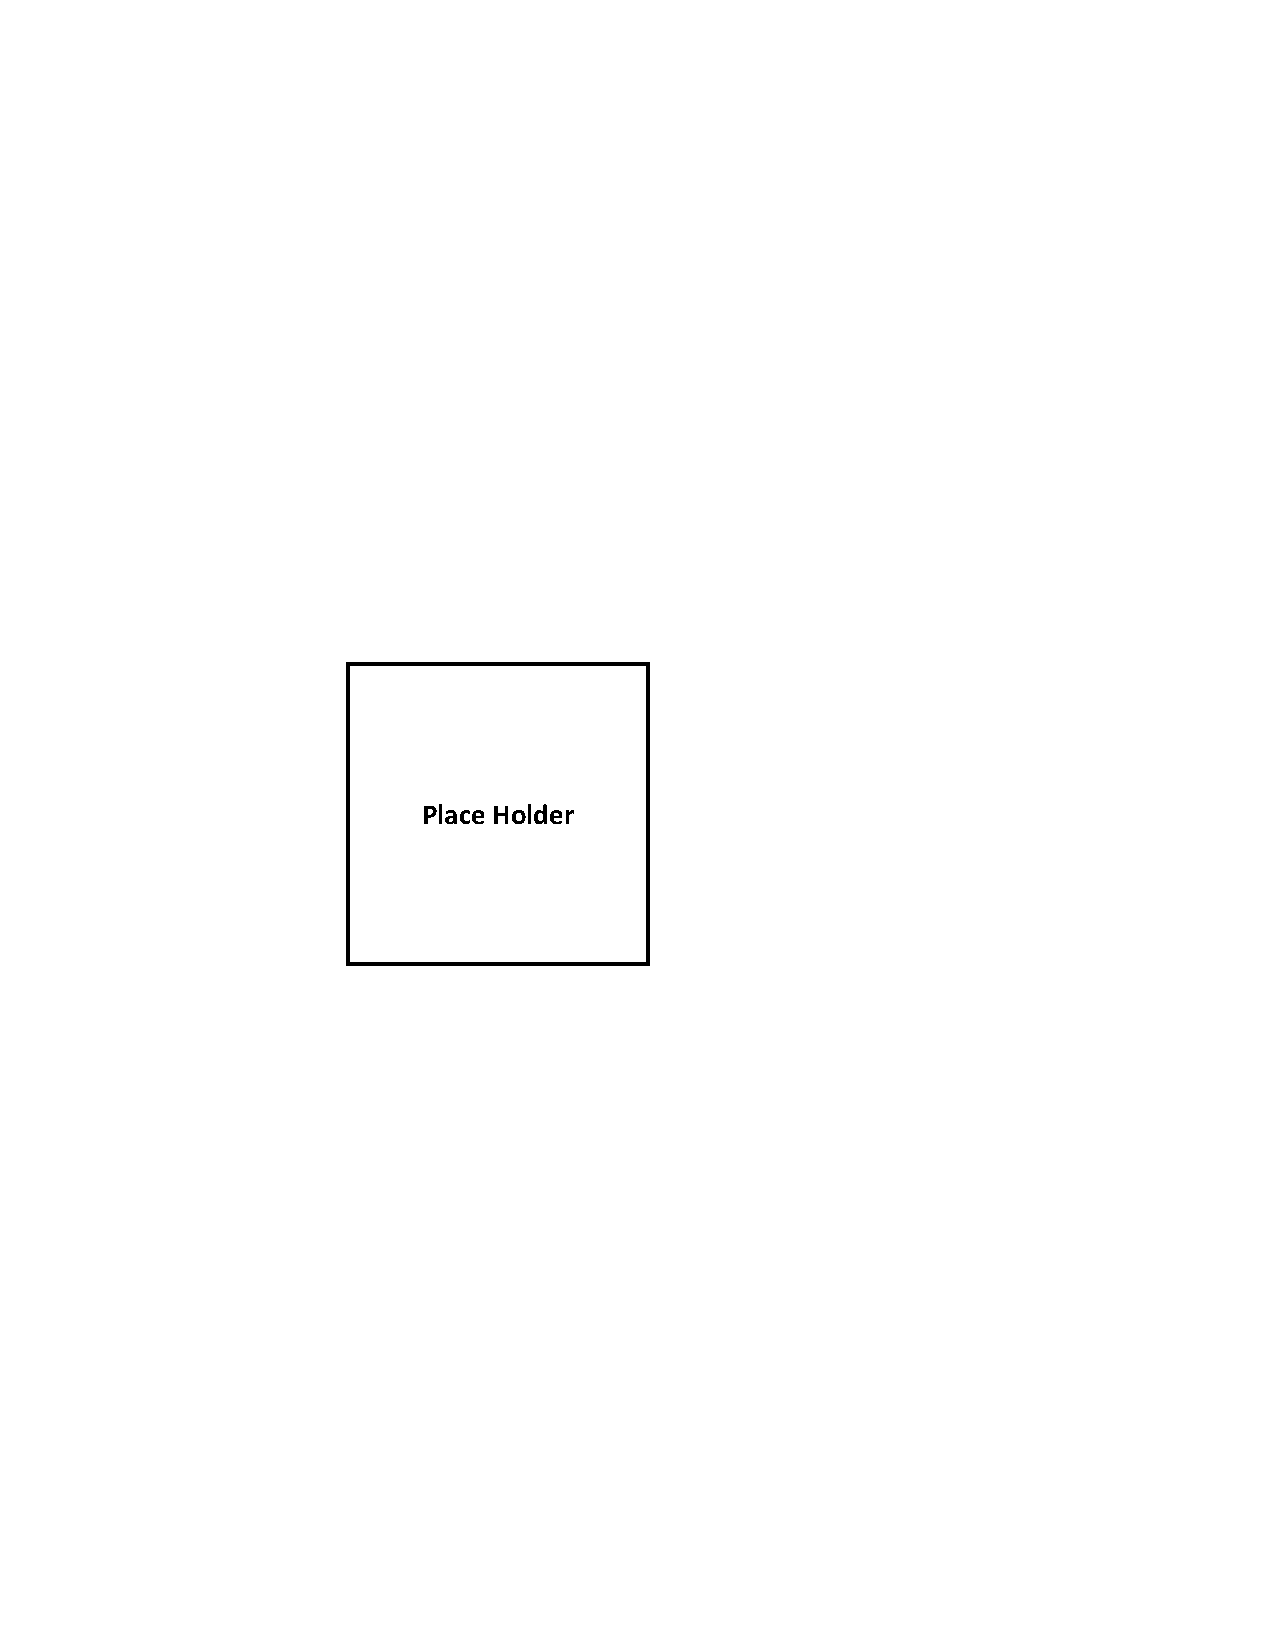
\includegraphics[width=\linewidth]{fig/PlaceHolder.pdf}
		\centerline{\dsreddit}
	\end{minipage}
	\hfill
	\begin{minipage}{0.18\linewidth}\centering
		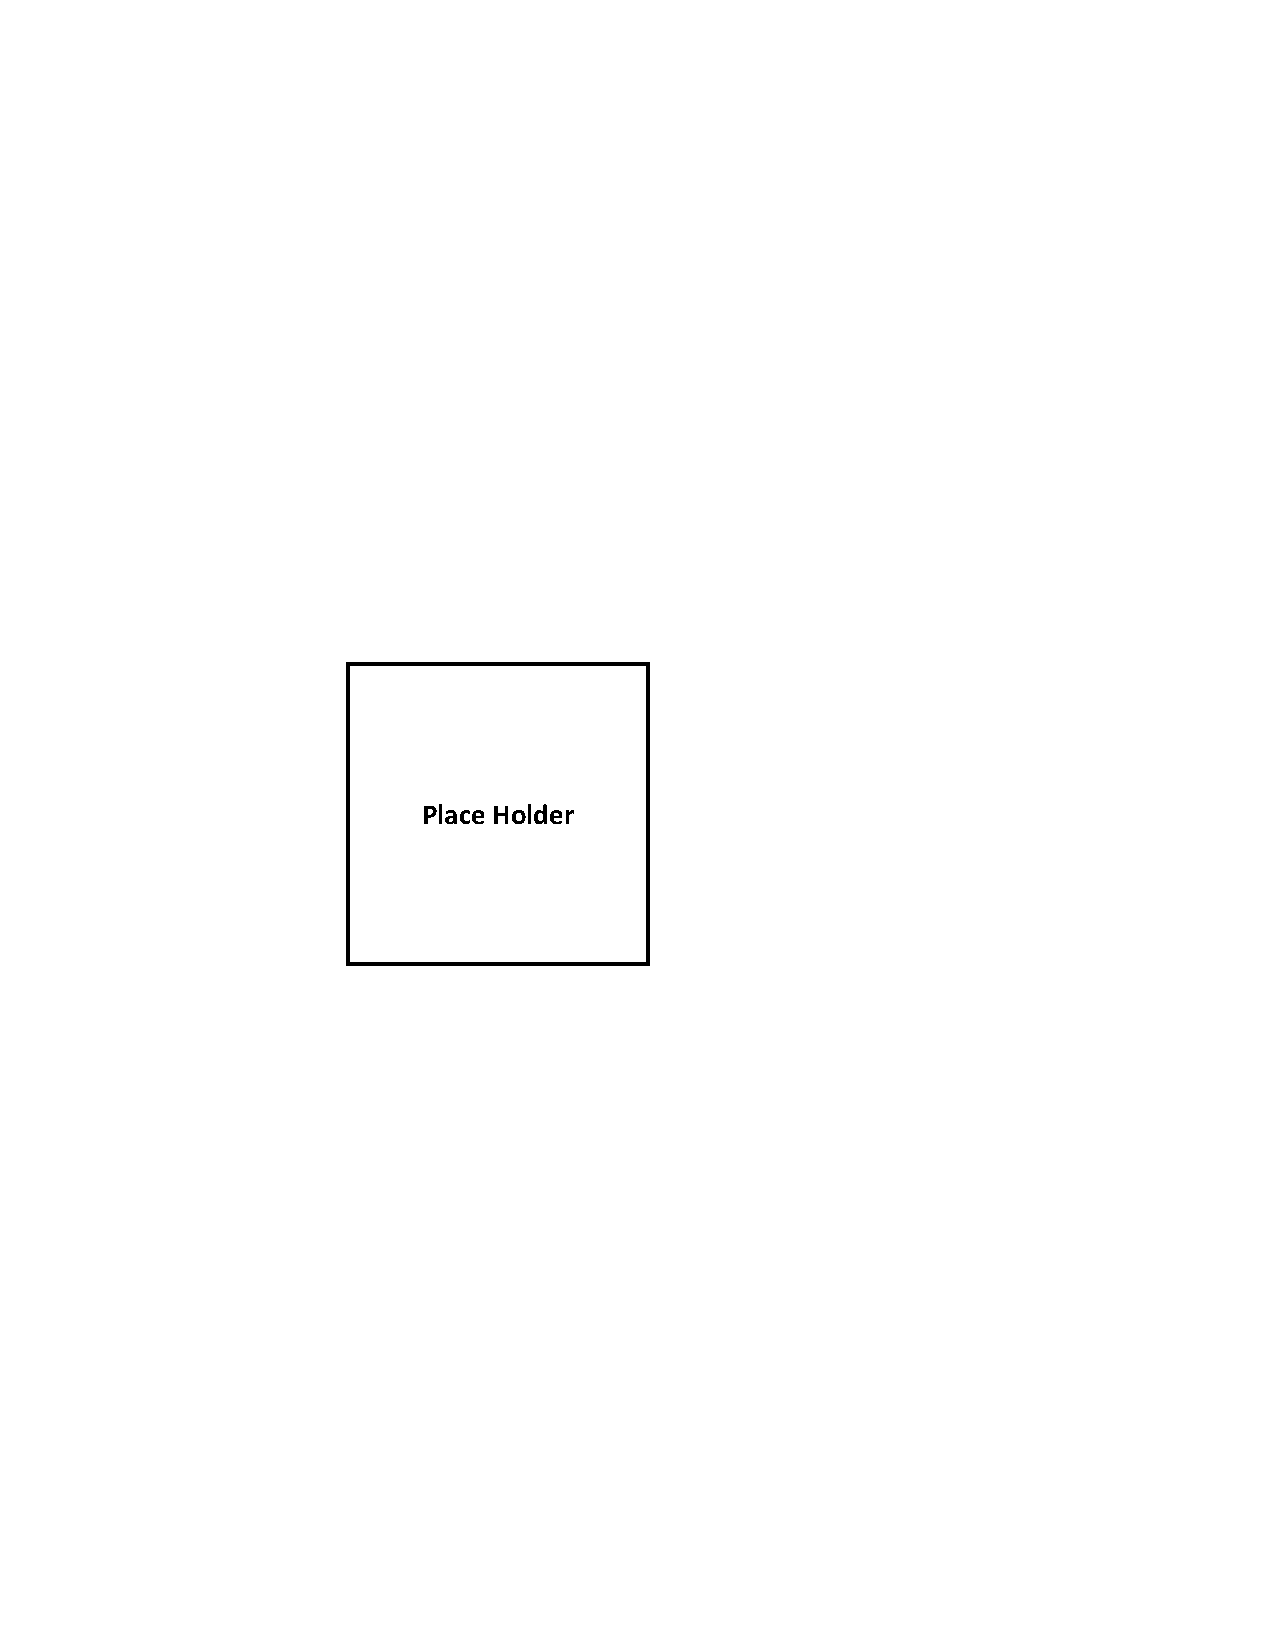
\includegraphics[width=\linewidth]{fig/PlaceHolder.pdf}
		\centerline{\dstpch}
	\end{minipage}
	\hfill
	\begin{minipage}{0.18\linewidth}\centering
		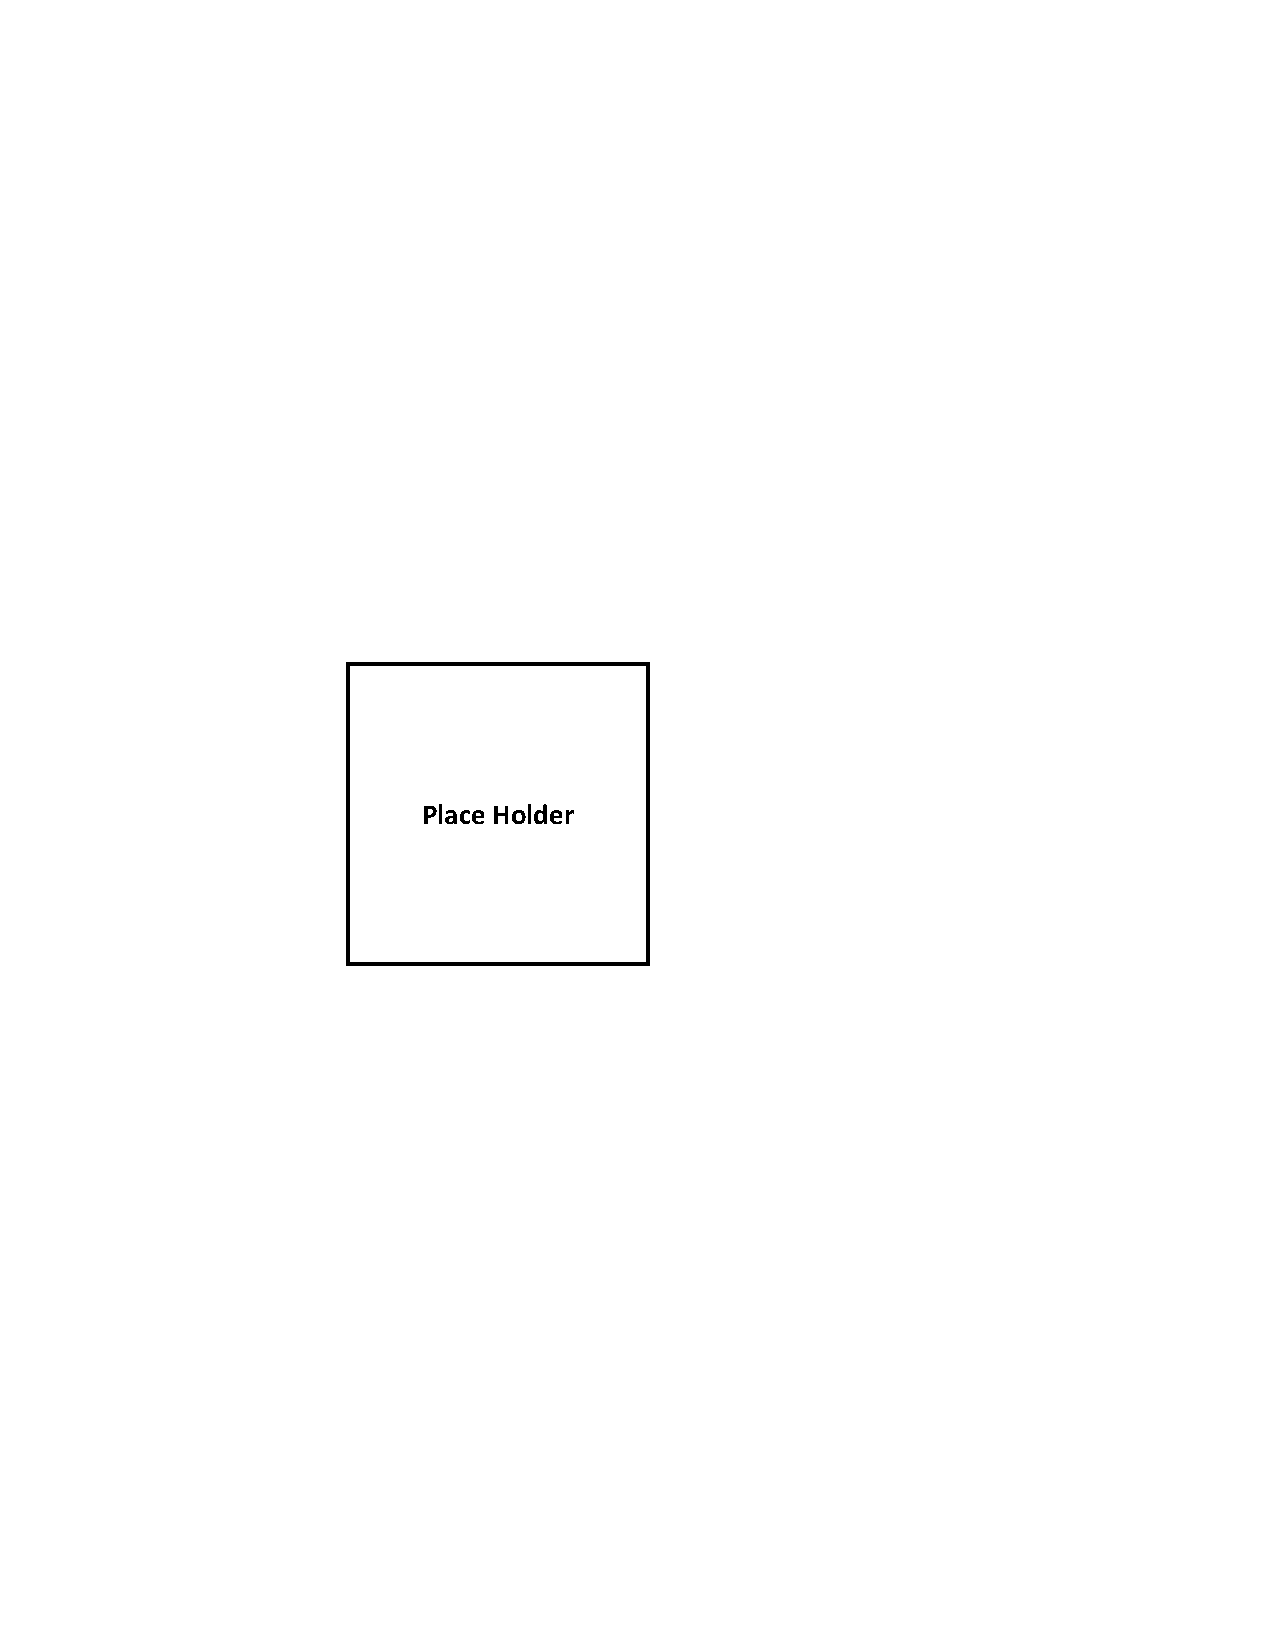
\includegraphics[width=\linewidth]{fig/PlaceHolder.pdf}
		\centerline{\dsali}
	\end{minipage}
	\hfill
	\begin{minipage}{0.18\linewidth}\centering
		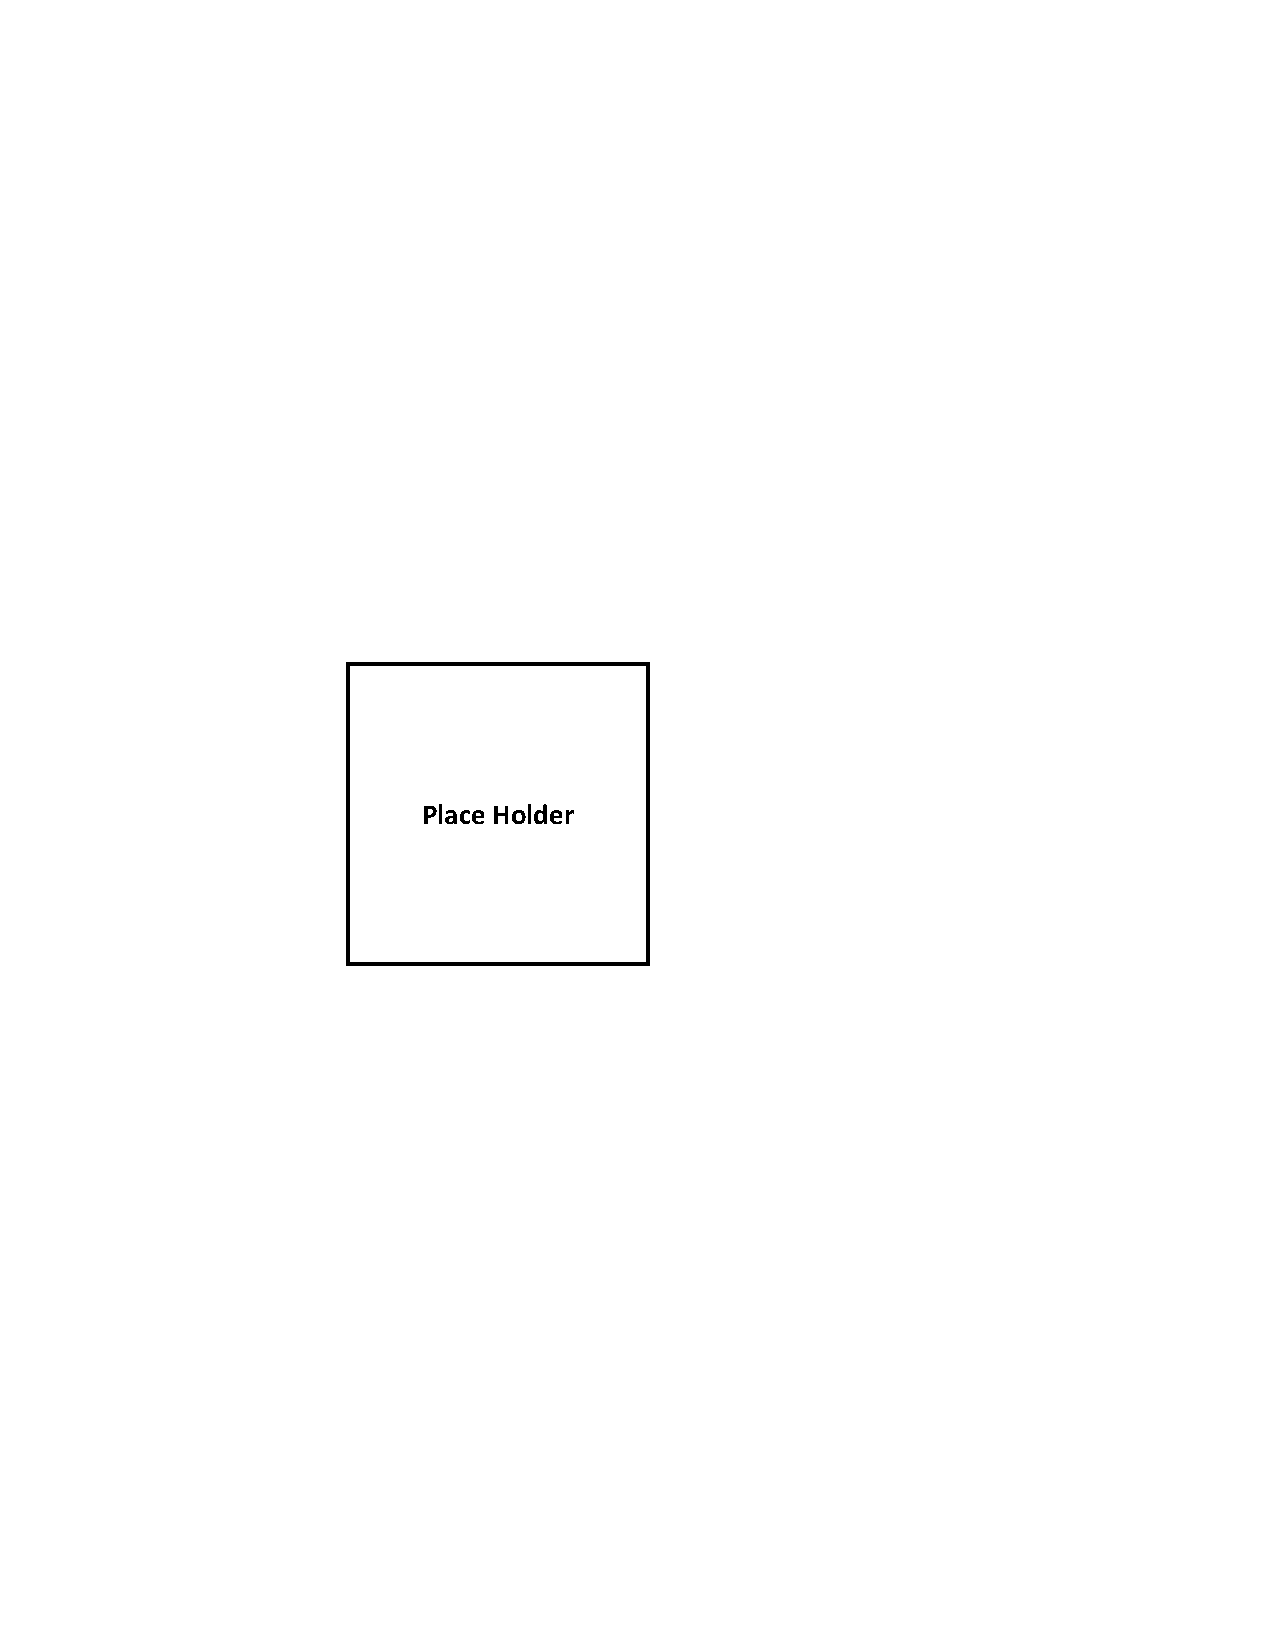
\includegraphics[width=\linewidth]{fig/PlaceHolder.pdf}
		\centerline{\dsrandom}
	\end{minipage}
	\caption{Run time for varying $r$.}
	\label{fig:vary-r-time}
\end{figure*}

\vspace{1mm}\noindent\textbf{Varying the batch size.}

\begin{figure*}[h]
	\begin{minipage}{0.18\linewidth}\centering
		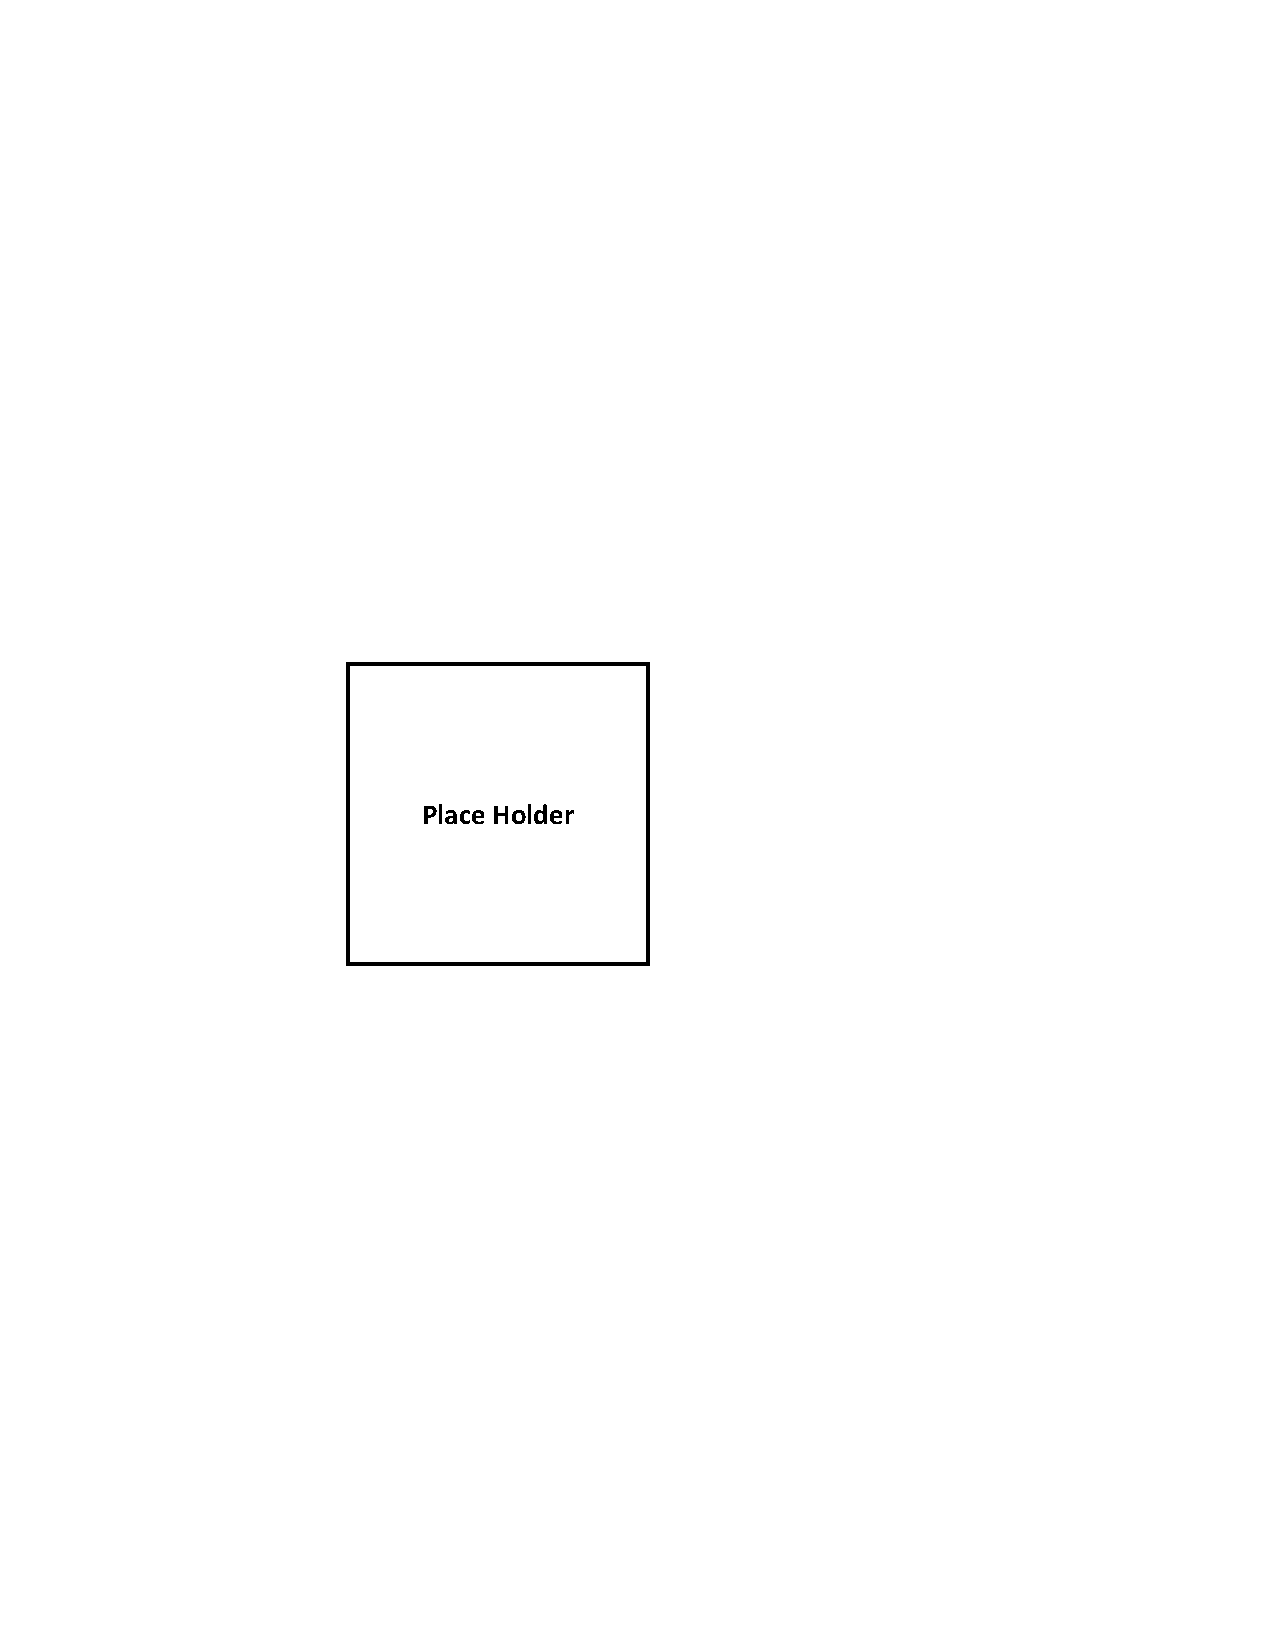
\includegraphics[width=\linewidth]{fig/PlaceHolder.pdf}
		\centerline{\dstwitter}
	\end{minipage}
	\hfill
	\begin{minipage}{0.18\linewidth}\centering
		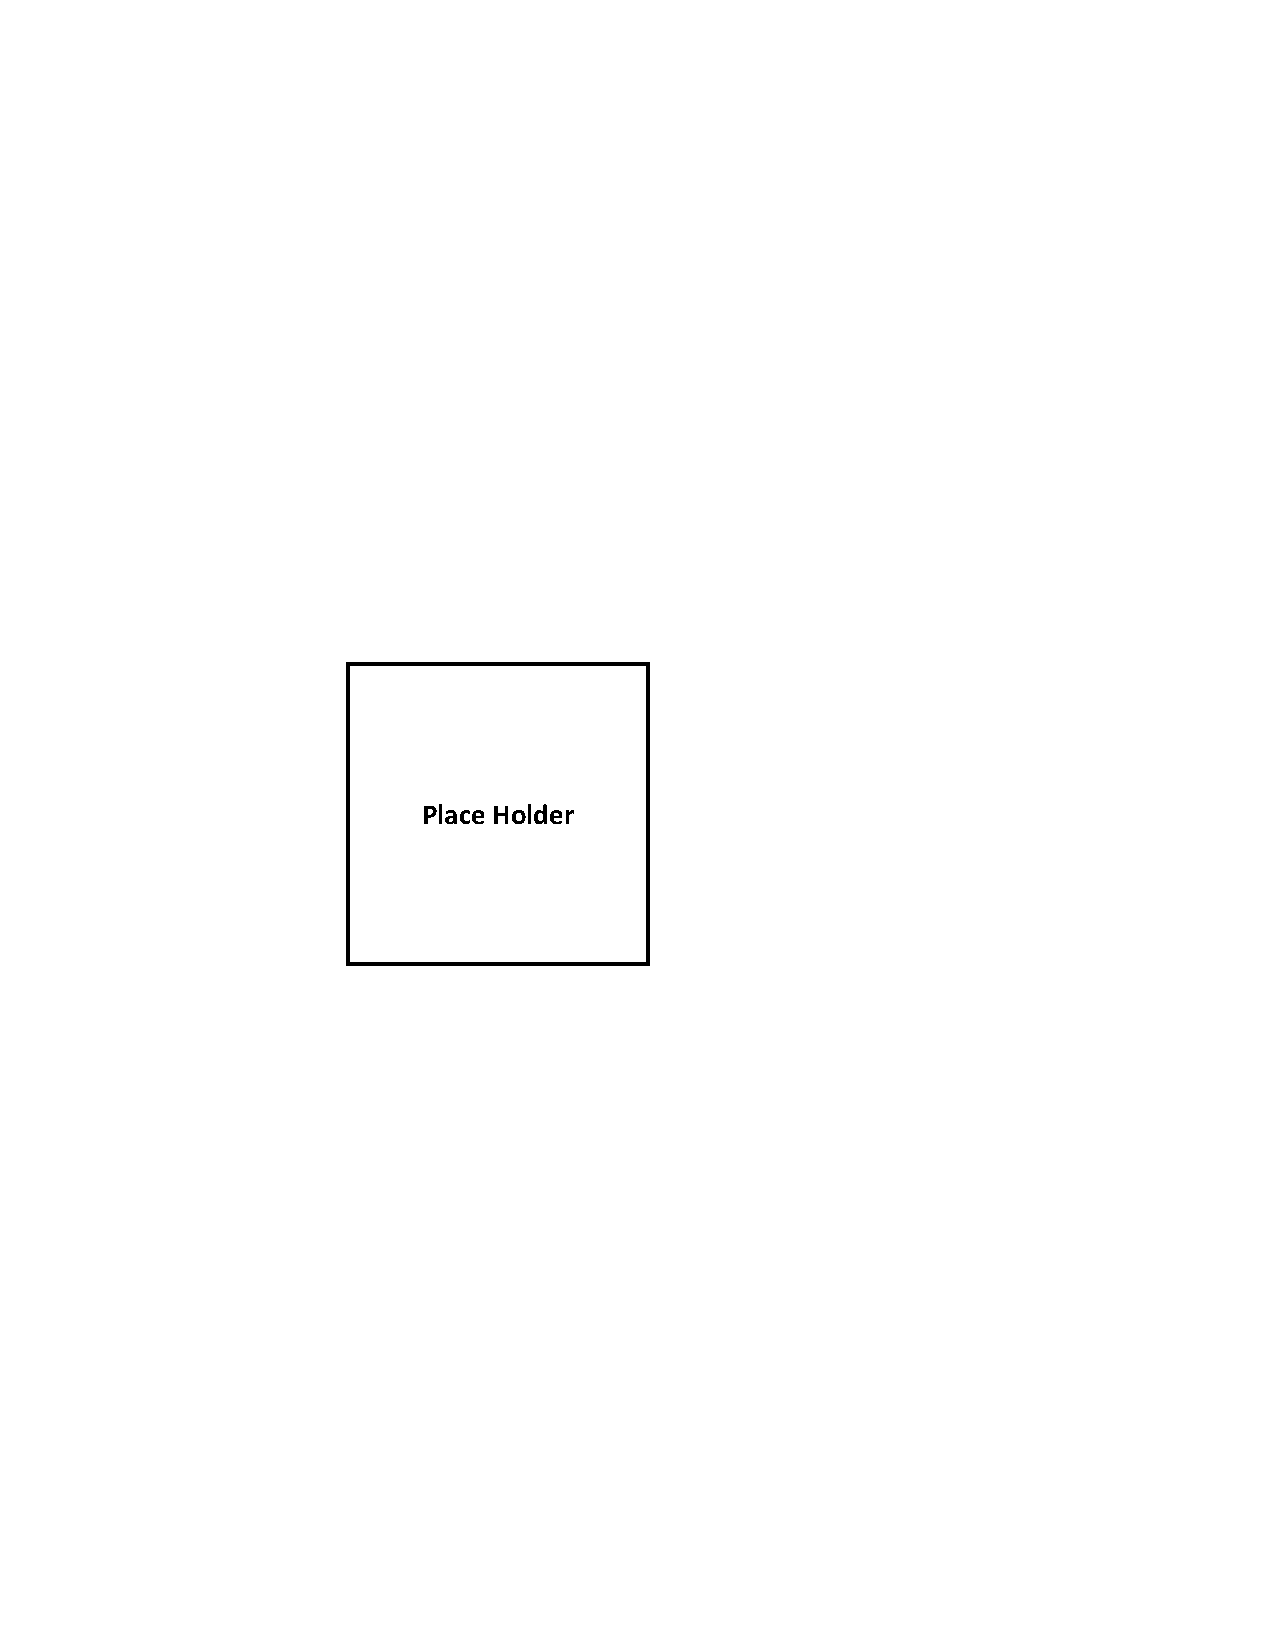
\includegraphics[width=\linewidth]{fig/PlaceHolder.pdf}
		\centerline{\dsreddit}
	\end{minipage}
	\hfill
	\begin{minipage}{0.18\linewidth}\centering
		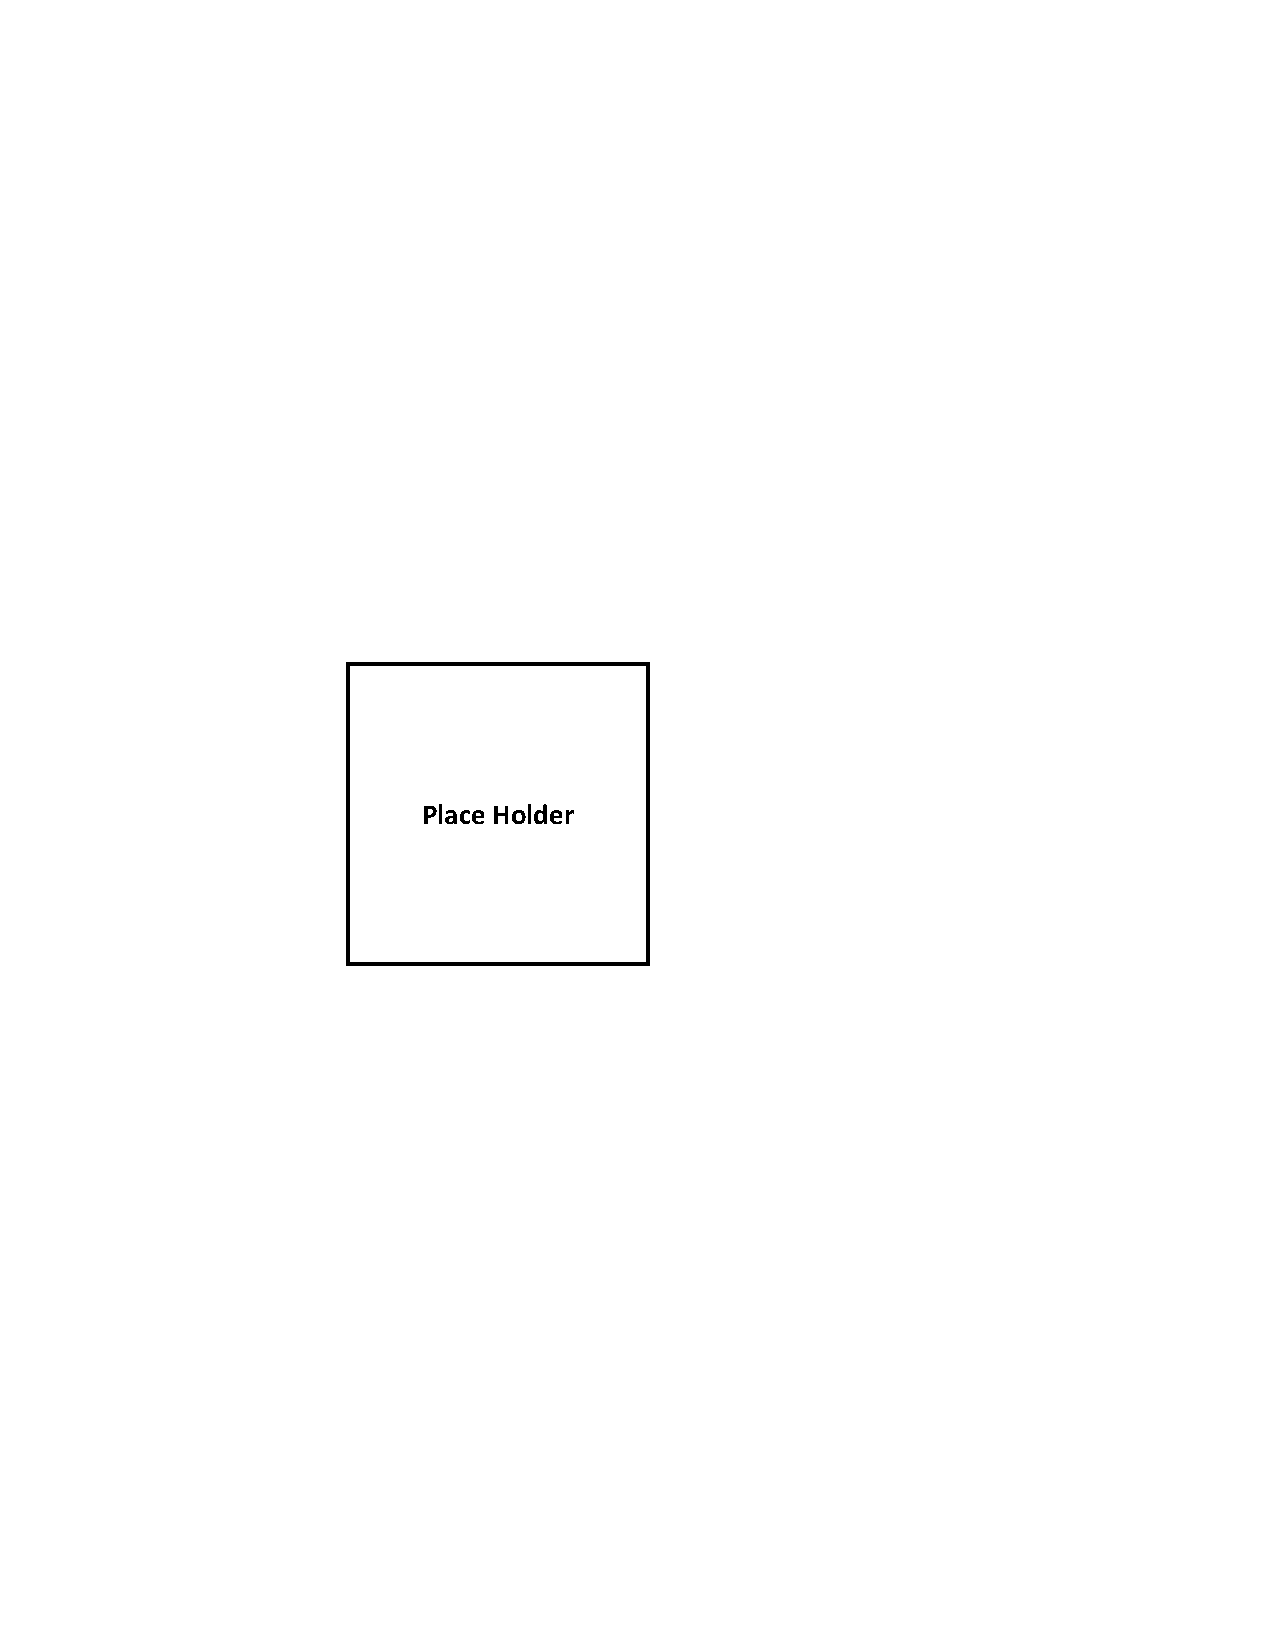
\includegraphics[width=\linewidth]{fig/PlaceHolder.pdf}
		\centerline{\dstpch}
	\end{minipage}
	\hfill
	\begin{minipage}{0.18\linewidth}\centering
		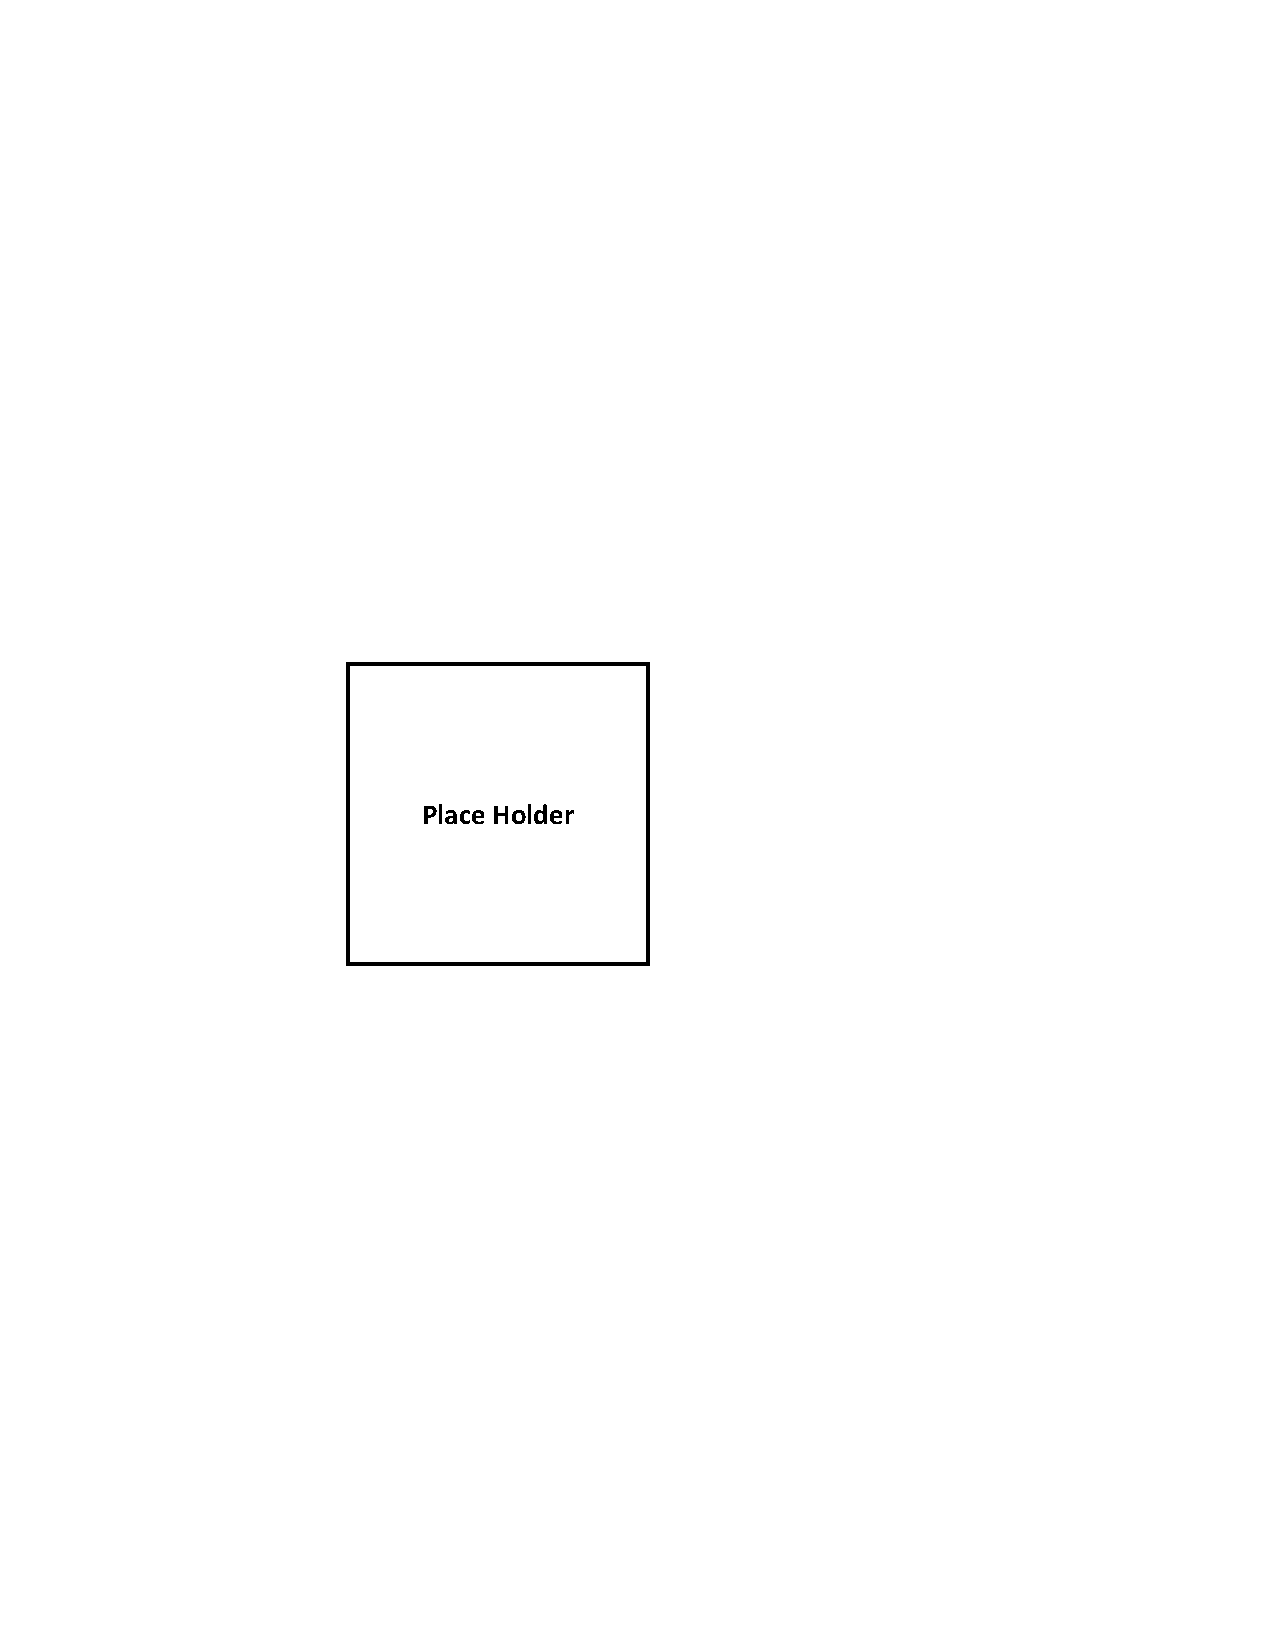
\includegraphics[width=\linewidth]{fig/PlaceHolder.pdf}
		\centerline{\dsali}
	\end{minipage}
	\hfill
	\begin{minipage}{0.18\linewidth}\centering
		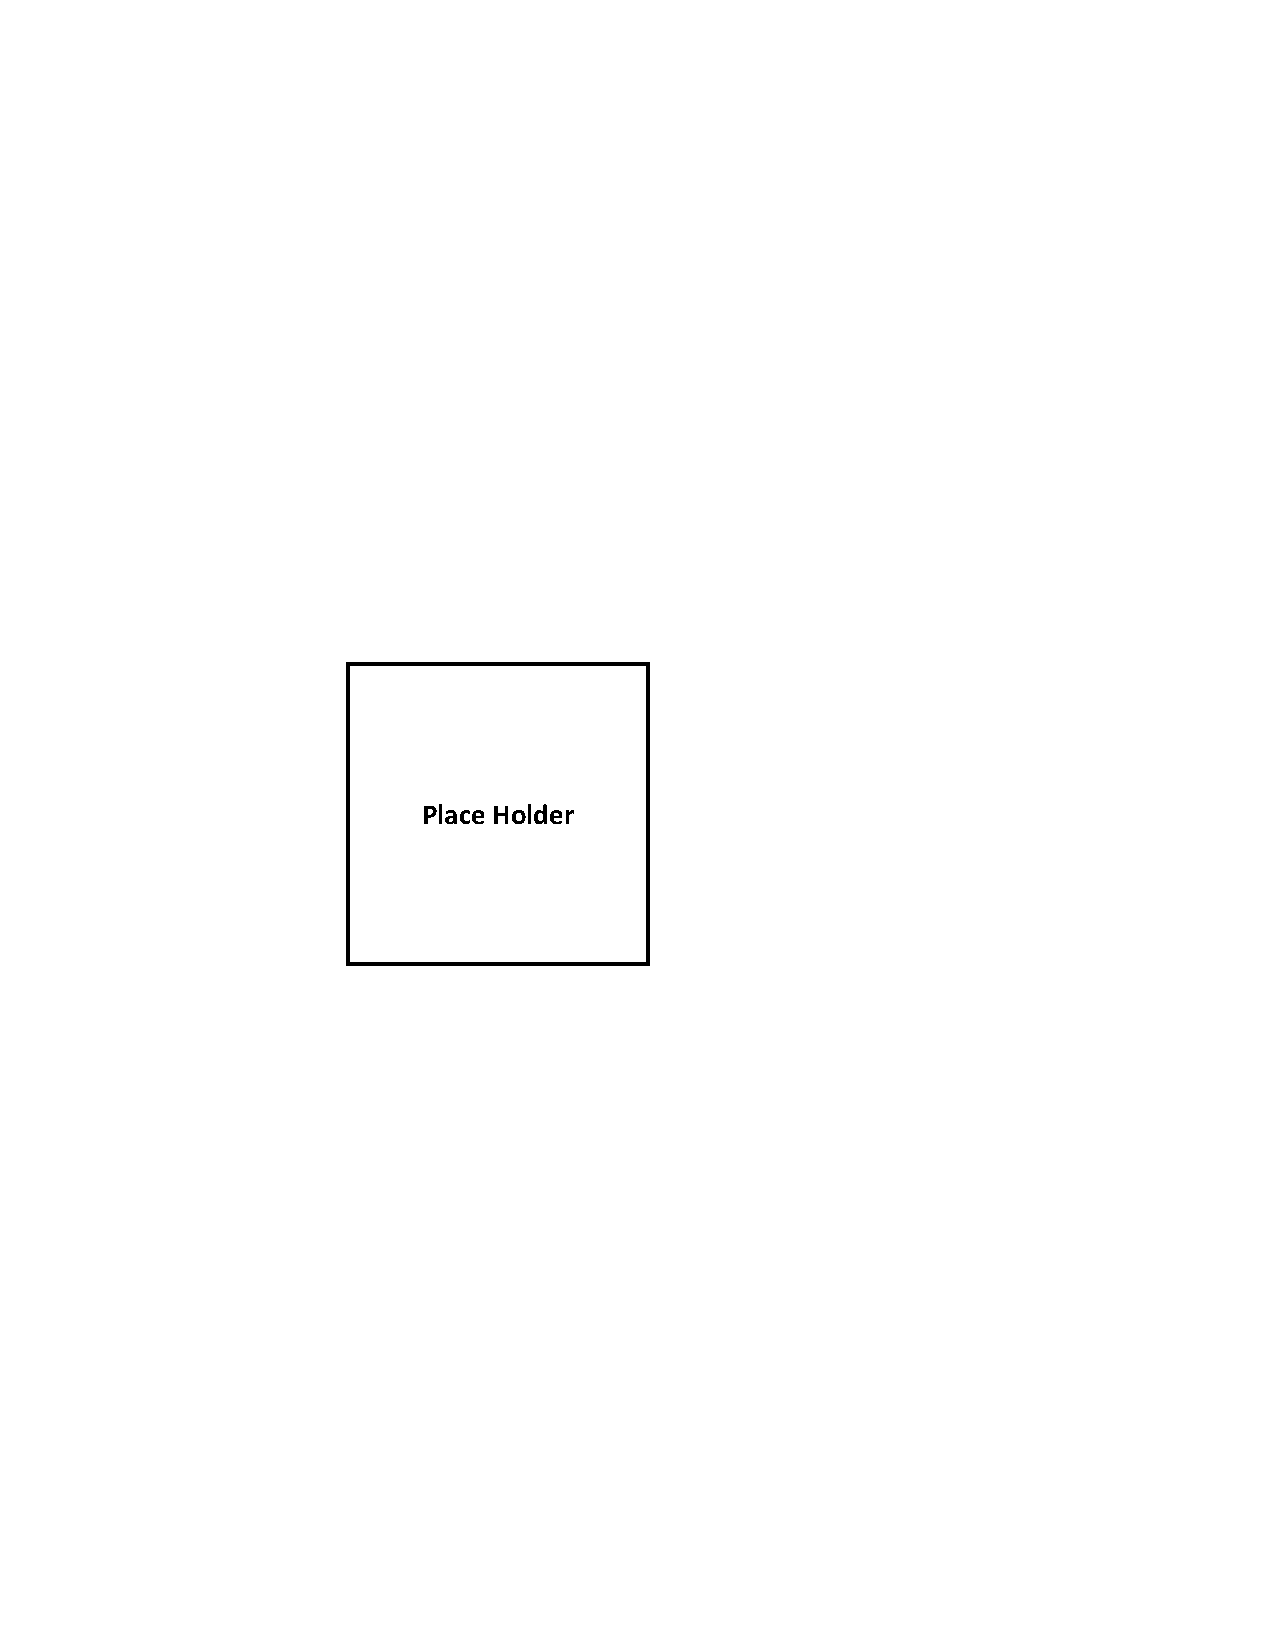
\includegraphics[width=\linewidth]{fig/PlaceHolder.pdf}
		\centerline{\dsrandom}
	\end{minipage}
	\caption{Run time for varying the batch size.}
	\label{fig:vary-batch-size}
\end{figure*}
